\chapter{Dataset}

This chapter describes the used datasets, including their construction methodologies. Since the perfomance of change point detection algorithms can be impacted by the time series attributes, it is made a brief analysis of the packet loss measurements. Also, it is presented an exploratory study of the change points dataset, which provides a further analysis of the problem difficulty. 

\section{End-to-End Packet Loss Fraction Time Series Dataset}

\subsection{Methodology}

The exposed time series of this work represent network end-to-end measures of a cable-television infrastructure, which runs DOCSIS with asymmetric download and upload bandwidths. Home routers connected to the cable modem communicate with one or more servers strategically located by the ISP. Measurements results from each home router are consolidated every half hour and, by the end of every day, are transferred to a database. The software responsible for these procedures was developed by TGR (a startup at COPPE/UFRJ) in collaboration the university (UFRJ), and is spread over a customers subset of a major Brazilian ISP.

The focus of this section is to analyze the loss fraction. In \cite{a_preliminary_performance_measurement_study_of_residential_broadband_services_in_brazil}, a preliminary investigation of other metrics is presented. To measure the round trip packet loss fraction between the home router and the associated server, the home router sends a train of short UDP packets, and then the server bounces back them. The data here presented considers a train of 100 UDP packets of 32 bytes, separated by 1 millisecond.

The resulted time series are unevenly spaced due to a range of reasons. First, measurements are initiated only if the residential link is not under use by the ISP customer. Also, the client may have no Internet connection to start a measurement, or even be without electrical energy.

\subsection{Descriptive Analysis}

This section analysis considers the period from 01/may/2016 to 20/may/2016. It was selected every client in which all measures of this period occurred against the same server. It was also imposed that the home router and the server must belong to the same Brazilian state. These filters resulted in 1870 clients time series and 1537272 measures.

Figure~\ref{fig:loss_fraction_cdf_ccdf} presents the packet loss fraction CDF and CCDF of all the clients measures. It is possible to note that 93.2\% of the measures have zero losses.

\begin{figure}[H]
    \makebox[\linewidth][c]{%
        \centering
        \begin{subfigure}[b]{0.55\textwidth}
            \centering
            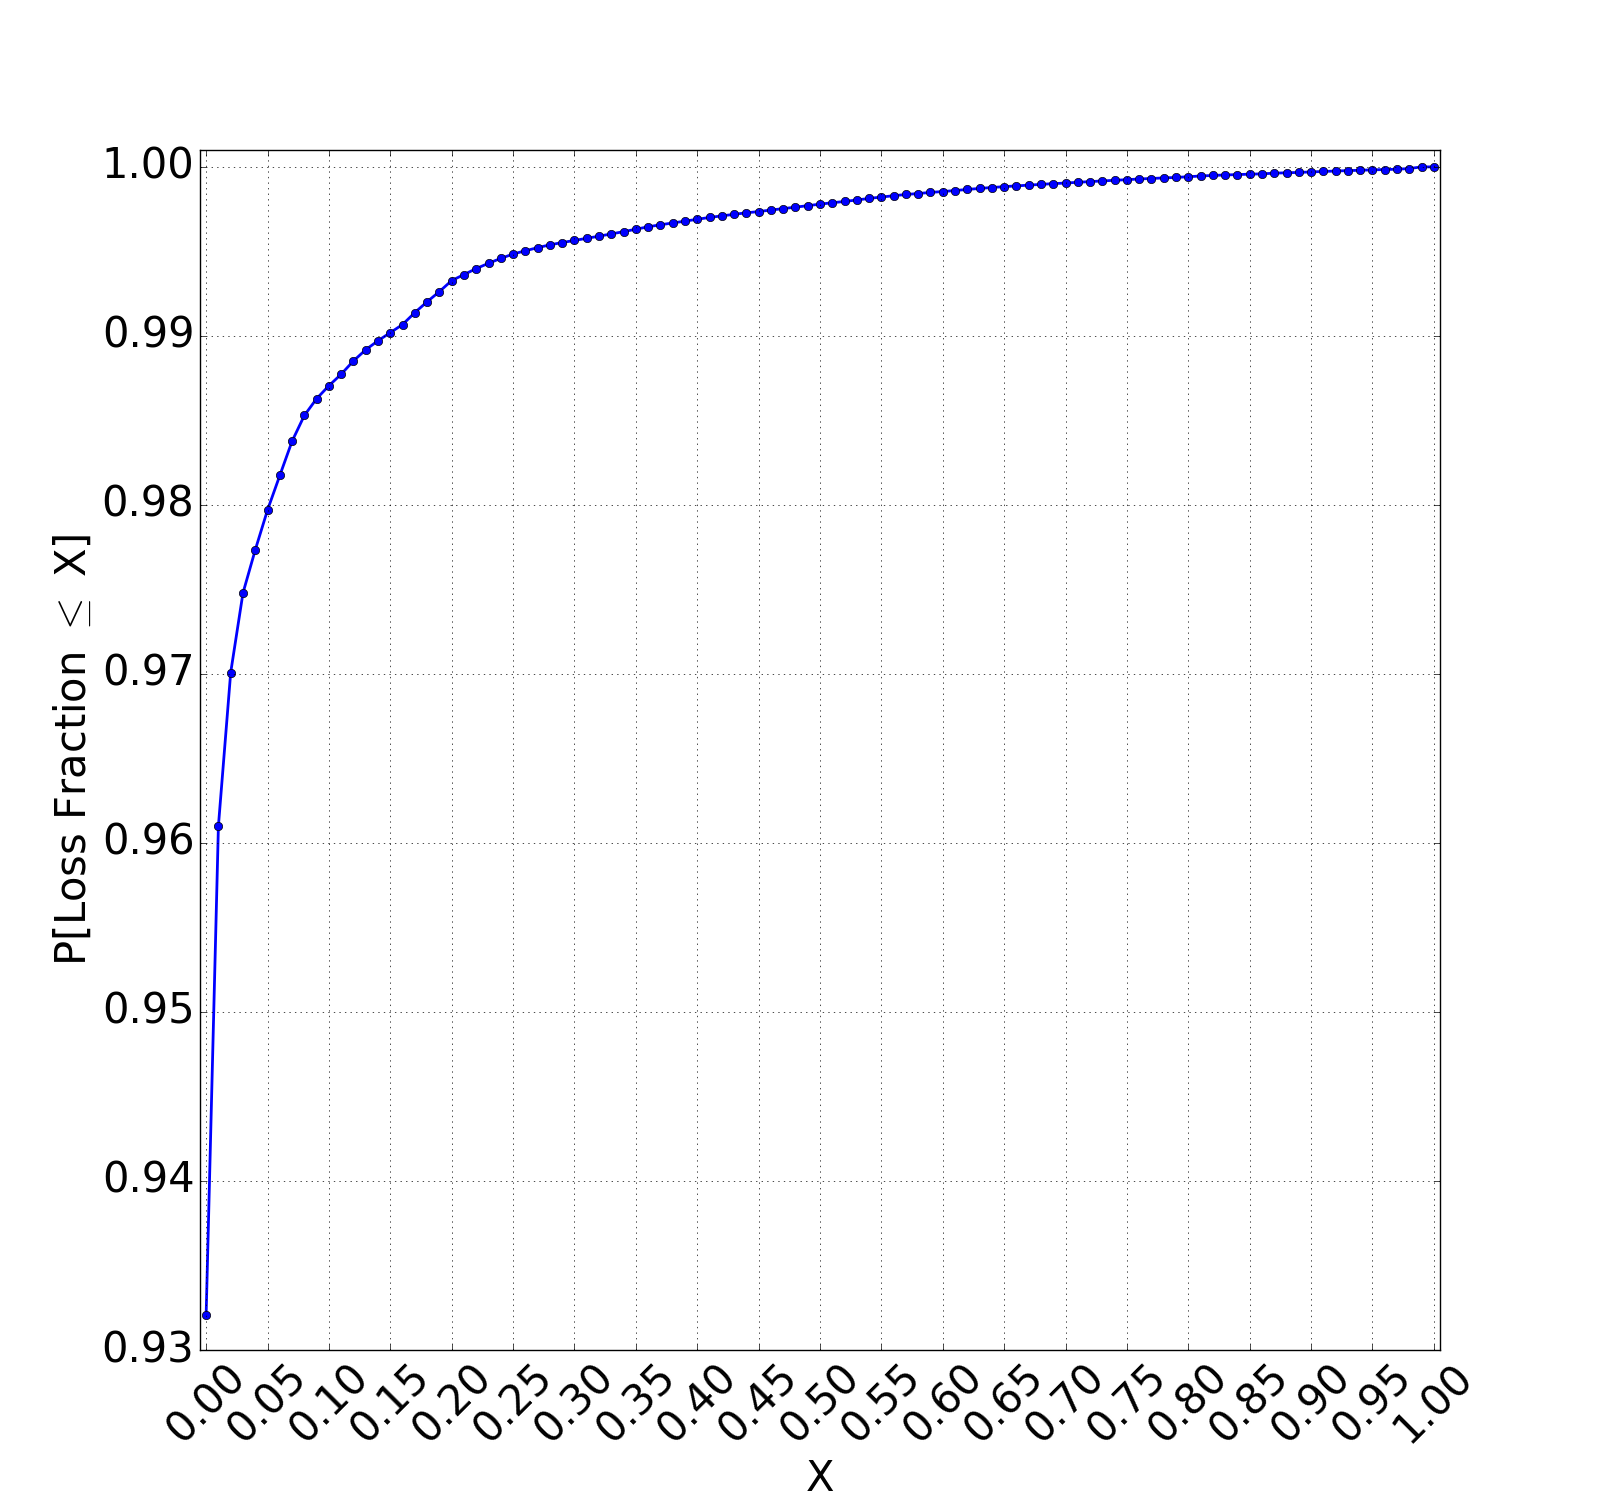
\includegraphics[width=\linewidth]{./figures/dataset/ts/cdf.png}
            \caption{CDF}
        \end{subfigure}%~
        \begin{subfigure}[b]{0.55\textwidth}
            \centering
            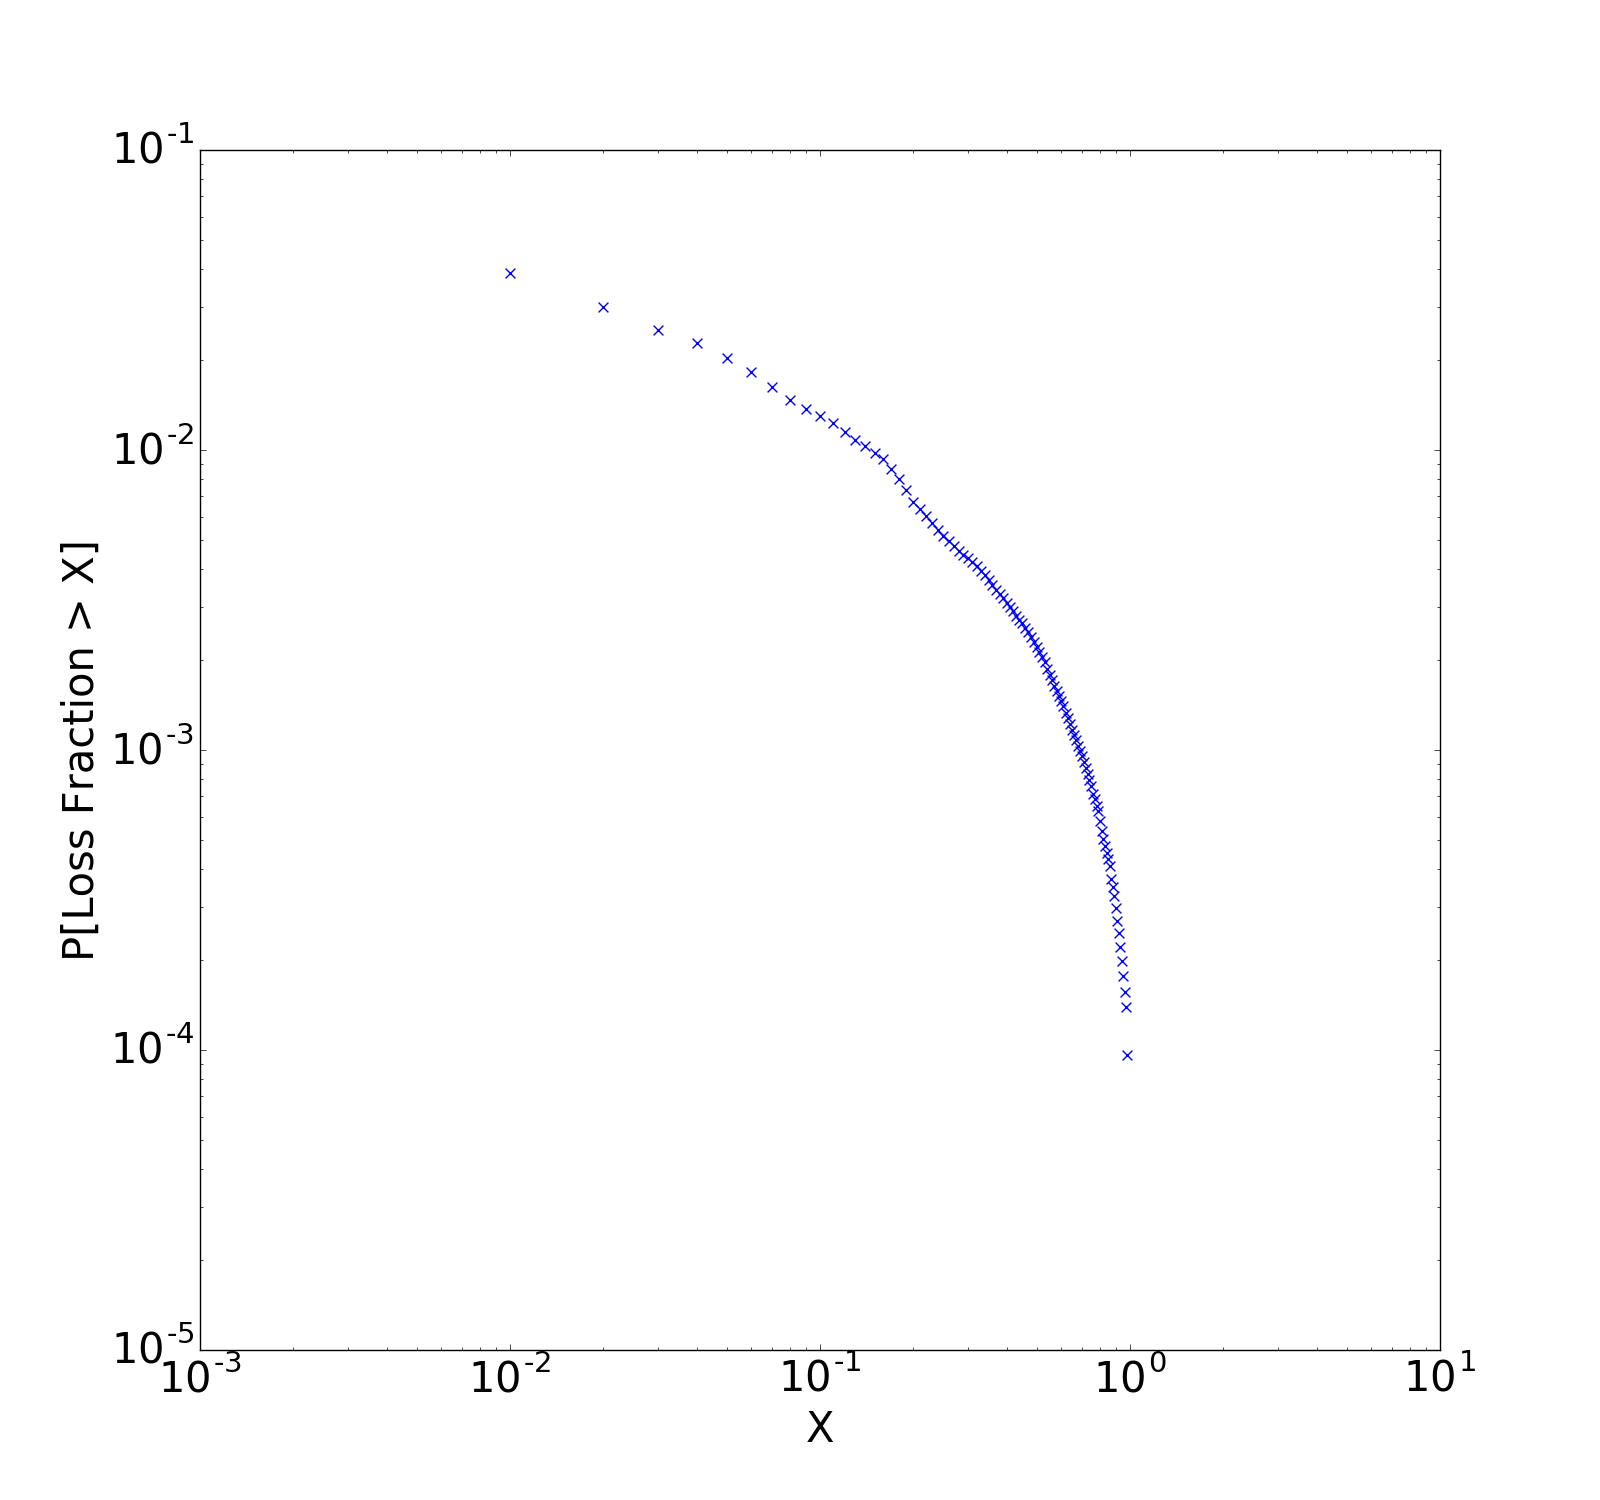
\includegraphics[width=\linewidth]{./figures/dataset/ts/ccdf.png}
            \caption{CCDF in log-log scale}
        \end{subfigure}
    }
    \caption{Packet Loss Fraction}
    \label{fig:loss_fraction_cdf_ccdf}
\end{figure}%

Figures~\ref{fig:loss_fraction_acf_ts_1},~\ref{fig:loss_fraction_acf_ts_2},~\ref{fig:loss_fraction_acf_ts_3} are examples of common autocorrelation patterns in this dataset. Since the data streams are unevenly spaced, it was considered only the date and hour components to compute the autocorrelation function. Therefore, if more than one measure occurred at the same hour and date, it was taken the average of these samples.

\begin{figure}[H]
    \makebox[\linewidth][c]{%
        \centering
        \begin{subfigure}[b]{0.55\textwidth}
            \centering
            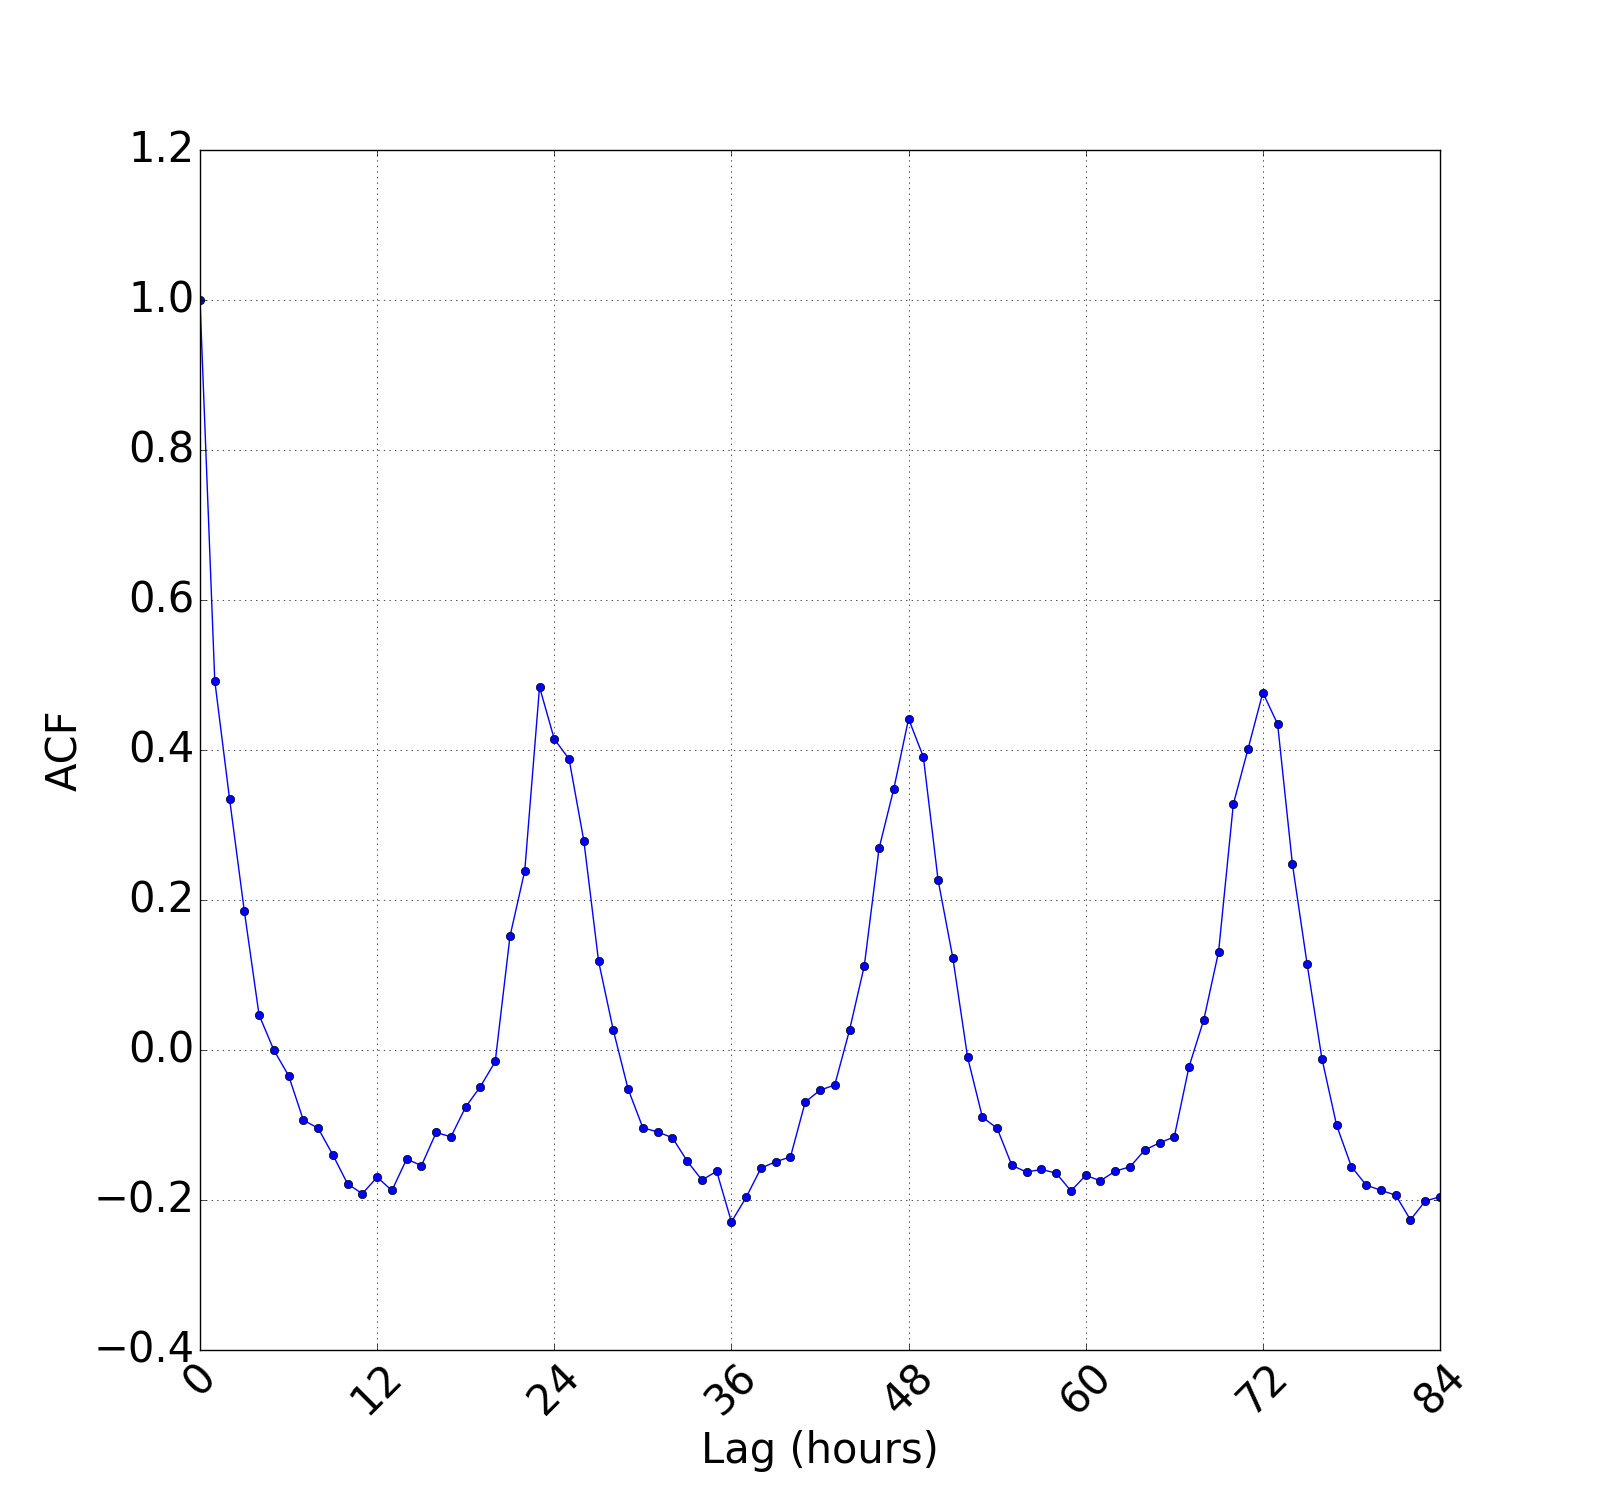
\includegraphics[width=\linewidth]{./figures/dataset/ts/acf_NHODTCSRV04_64:66:B3:50:05:BC.png}
            \caption{Autocorrelation}
        \end{subfigure}%~
        \begin{subfigure}[b]{0.55\textwidth}
            \centering
            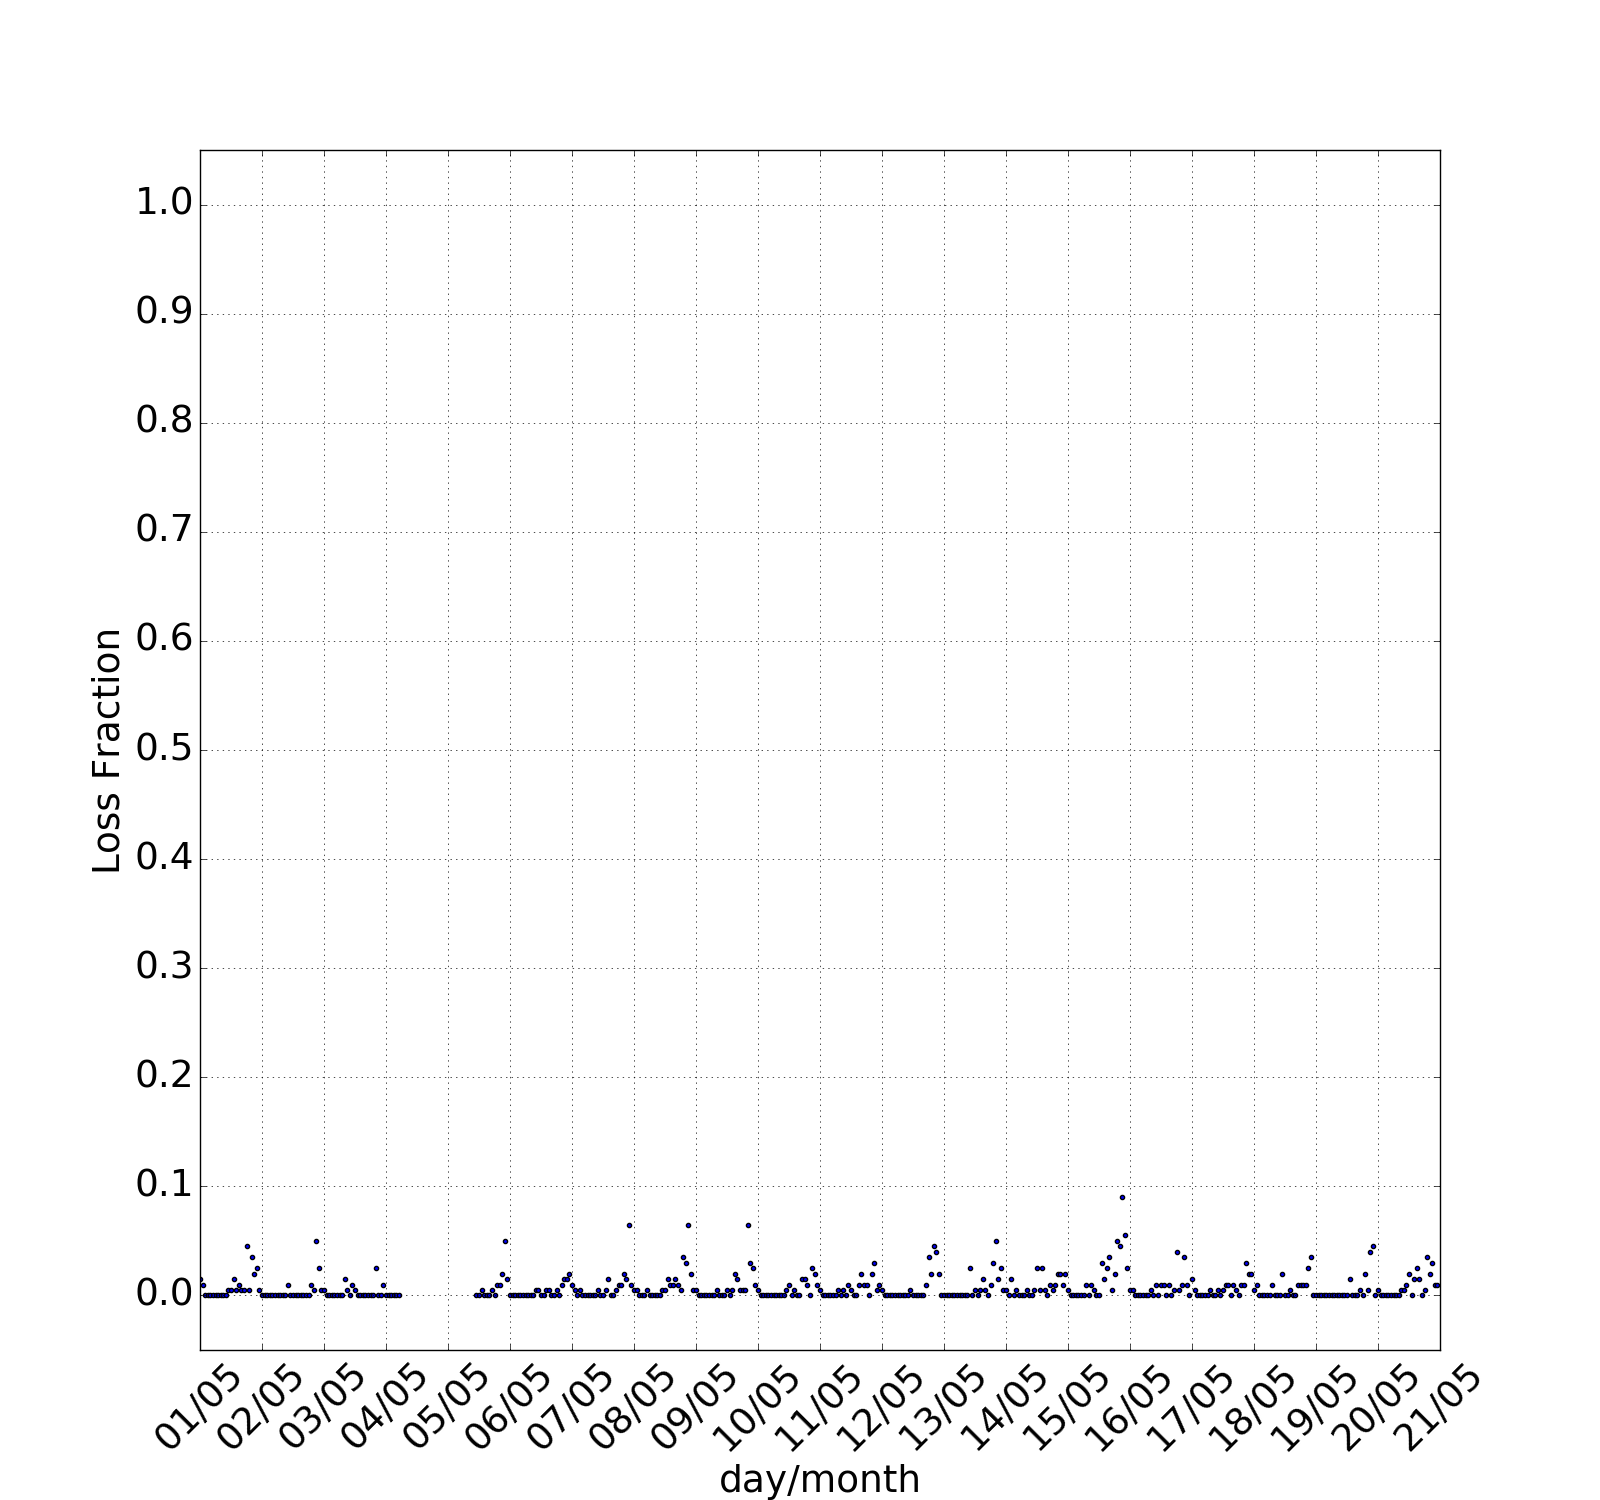
\includegraphics[width=\linewidth]{./figures/dataset/ts/ts_NHODTCSRV04_64:66:B3:50:05:BC.png}
            \caption{Time series}
        \end{subfigure}
    }
    \caption{Client 1}
    \label{fig:loss_fraction_acf_ts_1}
\end{figure}%

\begin{figure}[H]
    \makebox[\linewidth][c]{%
        \centering
        \begin{subfigure}[b]{0.55\textwidth}
            \centering
            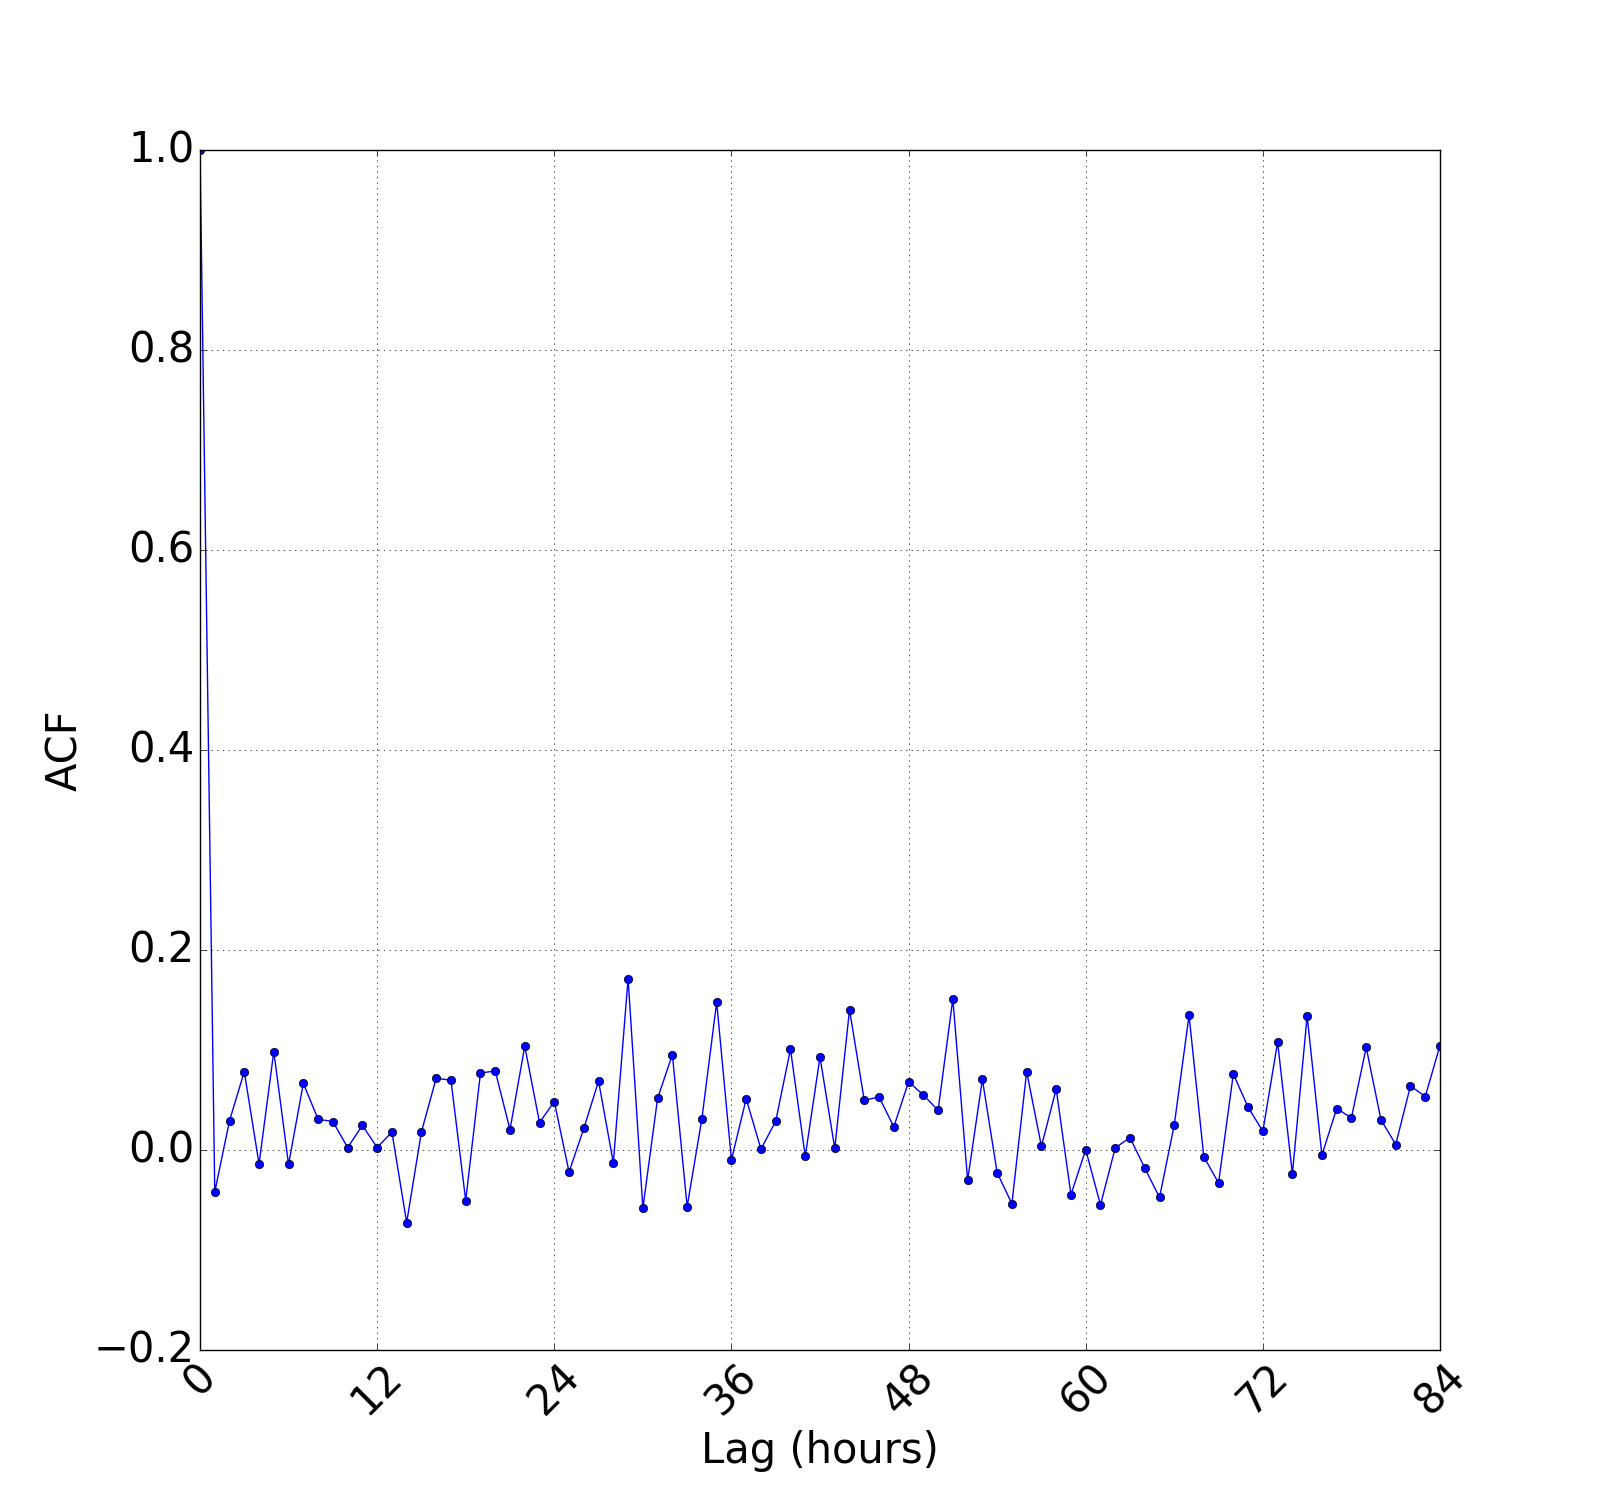
\includegraphics[width=1.0\textwidth]{./figures/dataset/ts/acf_BREDTCSRV20_64:66:B3:7B:9E:6A.png}
            \caption{Autocorrelation}
        \end{subfigure}%~
        \begin{subfigure}[b]{0.55\textwidth}
            \centering
            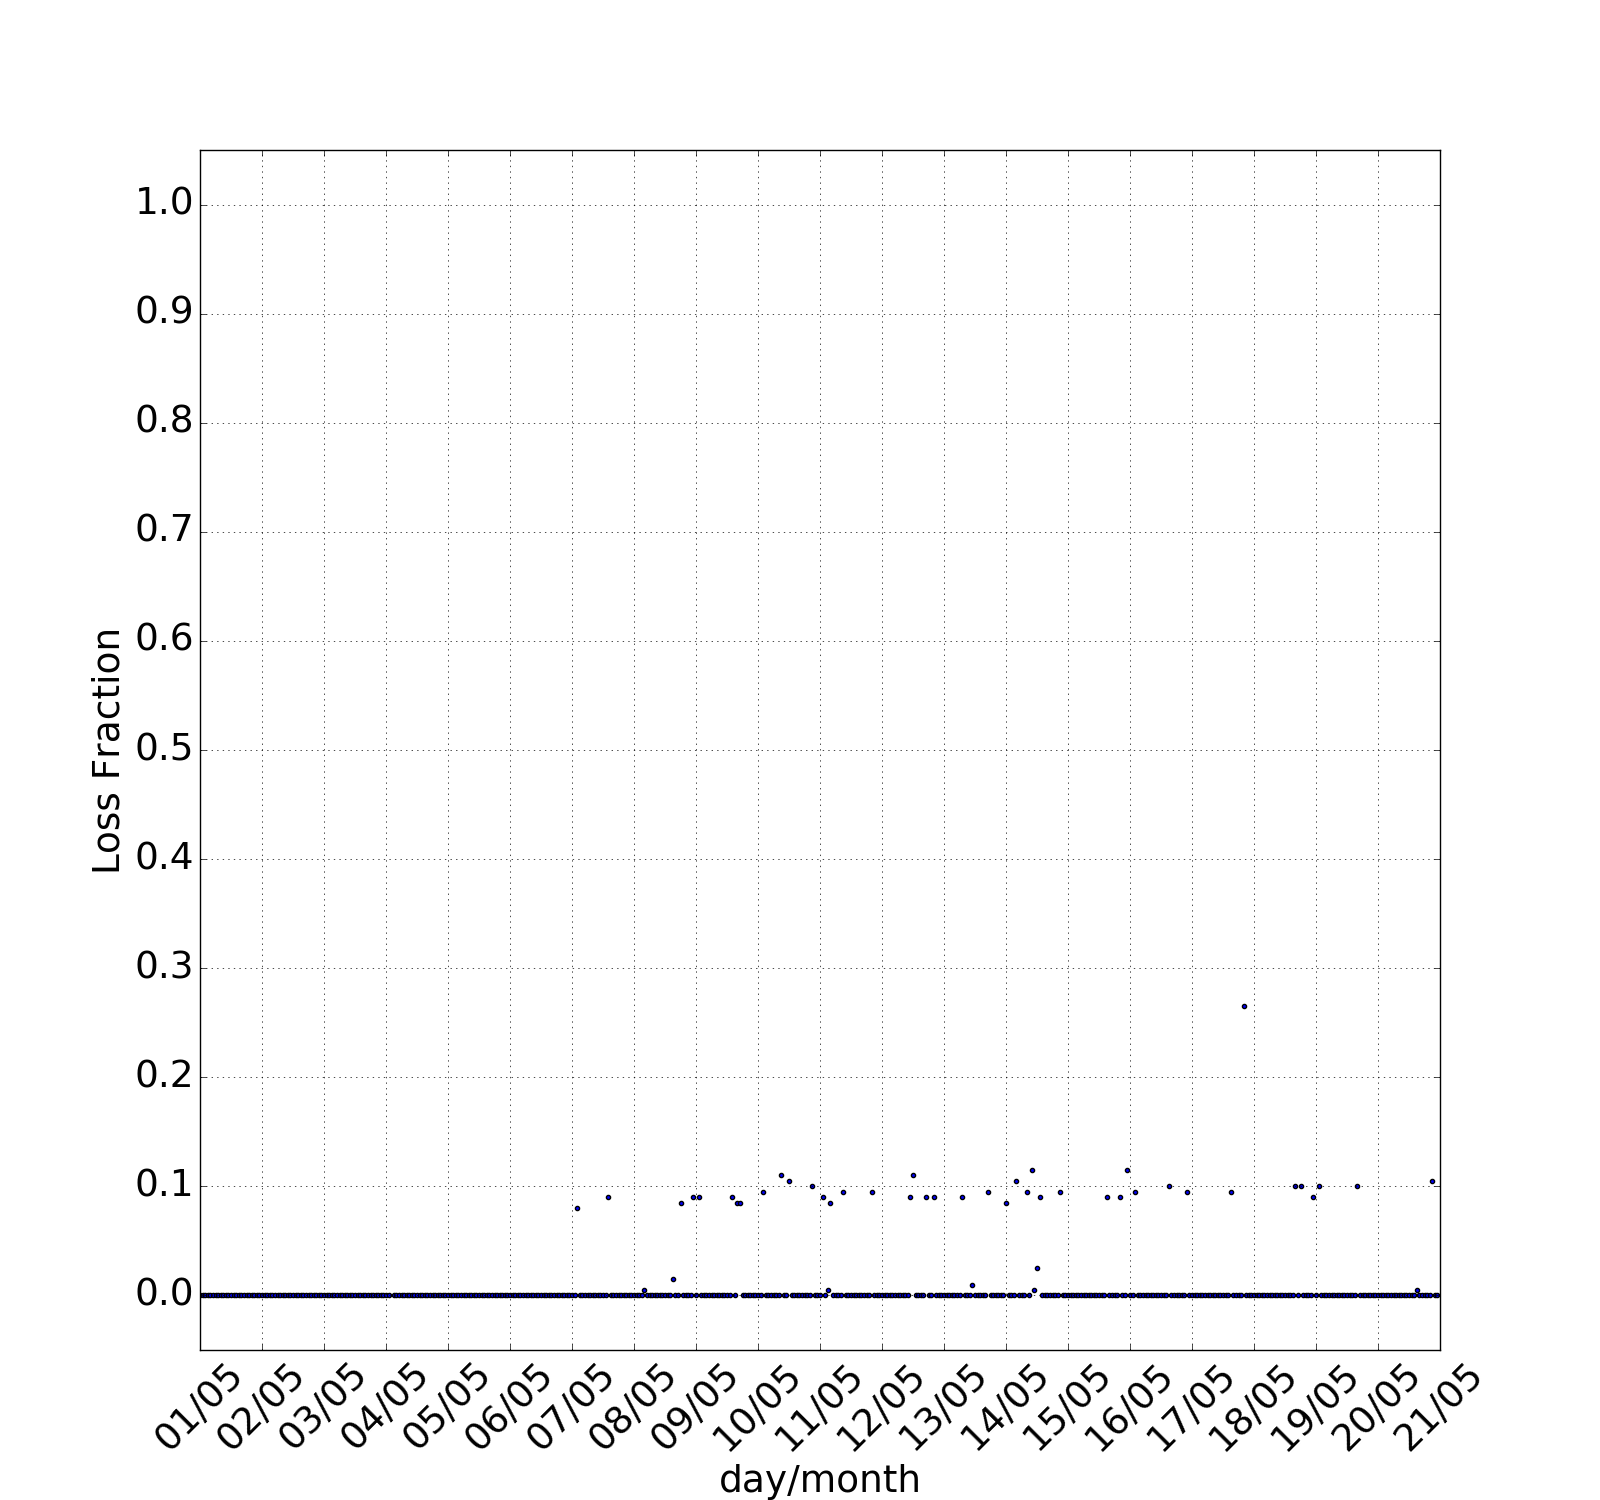
\includegraphics[width=1.0\textwidth]{./figures/dataset/ts/ts_BREDTCSRV20_64:66:B3:7B:9E:6A.png}
            \caption{Time series}
        \end{subfigure}
    }
    \caption{Client 2}
    \label{fig:loss_fraction_acf_ts_2}
\end{figure}

\begin{figure}[H]
    \makebox[\linewidth][c]{%
        \centering
        \begin{subfigure}[b]{0.55\textwidth}
            \centering
            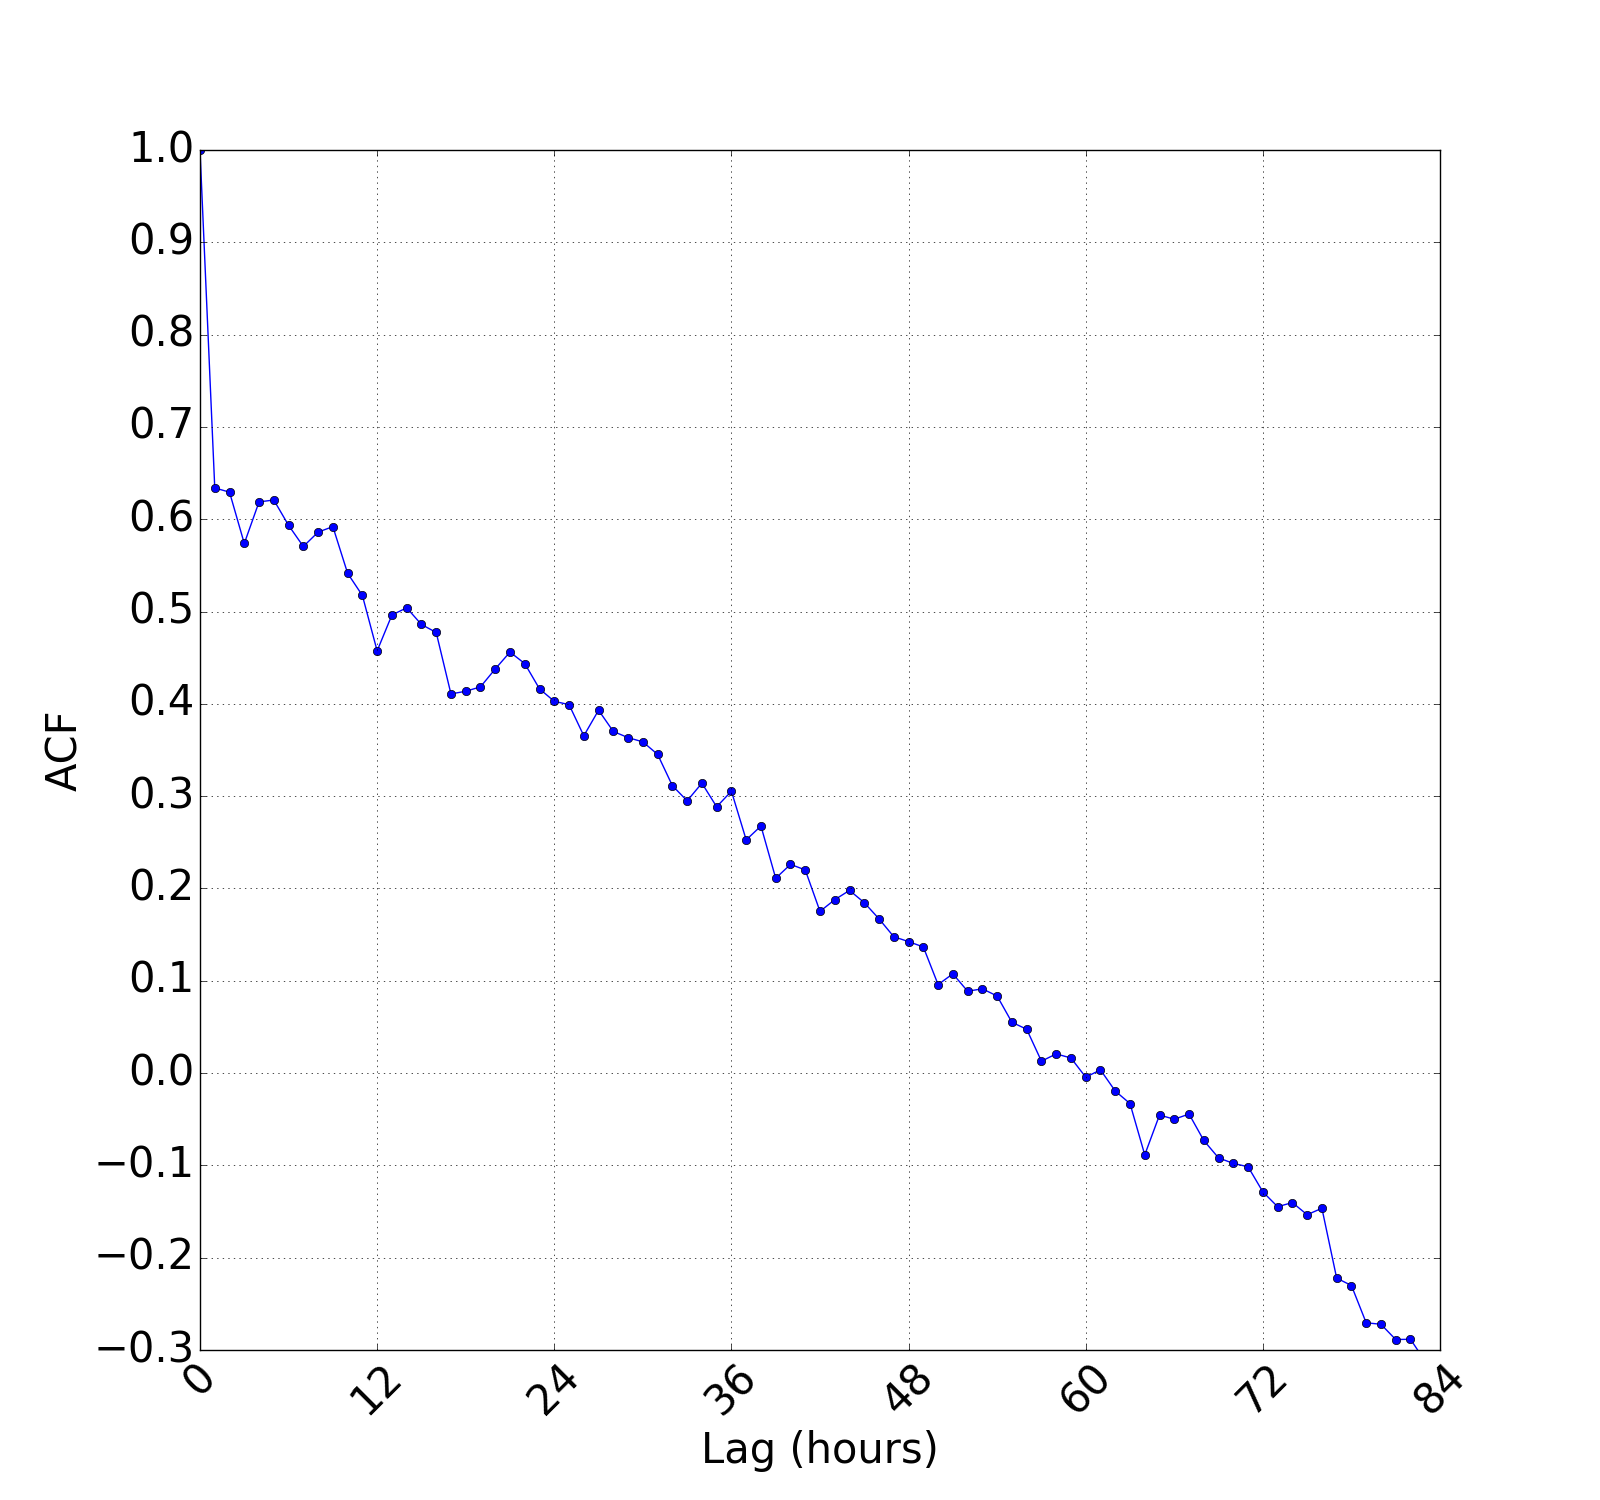
\includegraphics[width=1.0\textwidth]{./figures/dataset/ts/acf_BHZRENPEV01_64:66:B3:A6:BA:54.png}
            \caption{Autocorrelation}
        \end{subfigure}%~
        \begin{subfigure}[b]{0.55\textwidth}
            \centering
            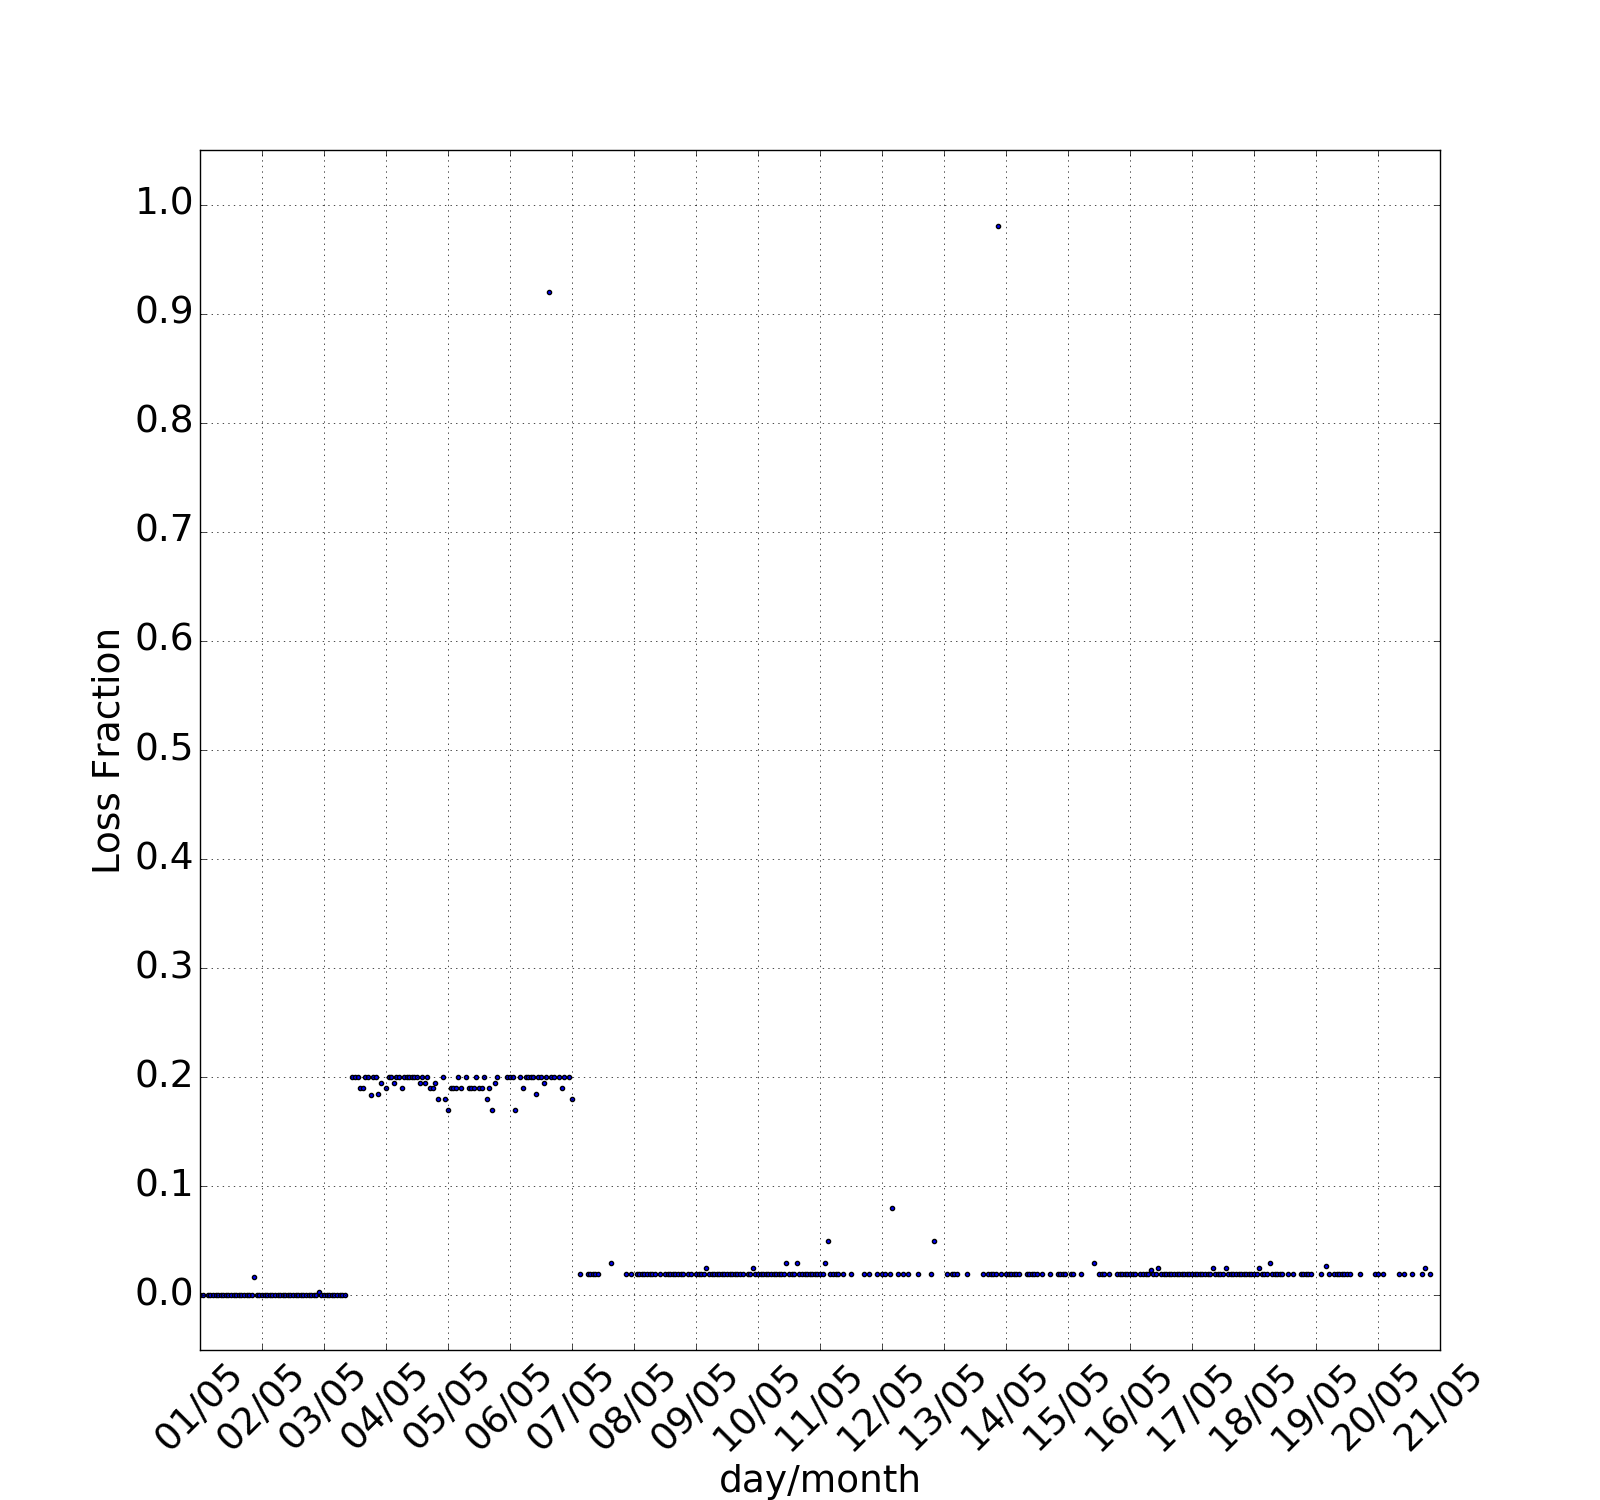
\includegraphics[width=1.0\textwidth]{./figures/dataset/ts/ts_BHZRENPEV01_64:66:B3:A6:BA:54.png}
            \caption{Time series}
        \end{subfigure}
    }
    \caption{Client 3}
    \label{fig:loss_fraction_acf_ts_3}
\end{figure}

The autocorrelation of Figure~\ref{fig:loss_fraction_acf_ts_1} have a periodic pattern, with peaks around multiples of 24 hours. In this client, it is possible to observe that losses are more usual at night. However, in Figure~\ref{fig:loss_fraction_acf_ts_2}, the autocorrelation quickly decreases and fluctuates around zero. The corresponding time series has a common characteristic, from 07/may on, measures with losses alternated with zero loss measures. Figure~\ref{fig:loss_fraction_acf_ts_3} shows a linear decreasing autocorrelation, and the associated time series presents abrupt changes in the mean.

As in Figure~\ref{fig:loss_fraction_acf_ts_1}, some clients have a daily pattern in which losses occur more frequently at night. This fact can be linked with congestion, since the Internet usage increases at the end of a day. Figure~\ref{fig:mean_day_hour_ts} corroborates that observation, illustrating the mean and variance of measures that occurred in a specific hour through all days.

\begin{figure}[H]
    \makebox[\linewidth][c]{%
        \centering
        \begin{subfigure}[b]{0.55\textwidth}
            \centering
            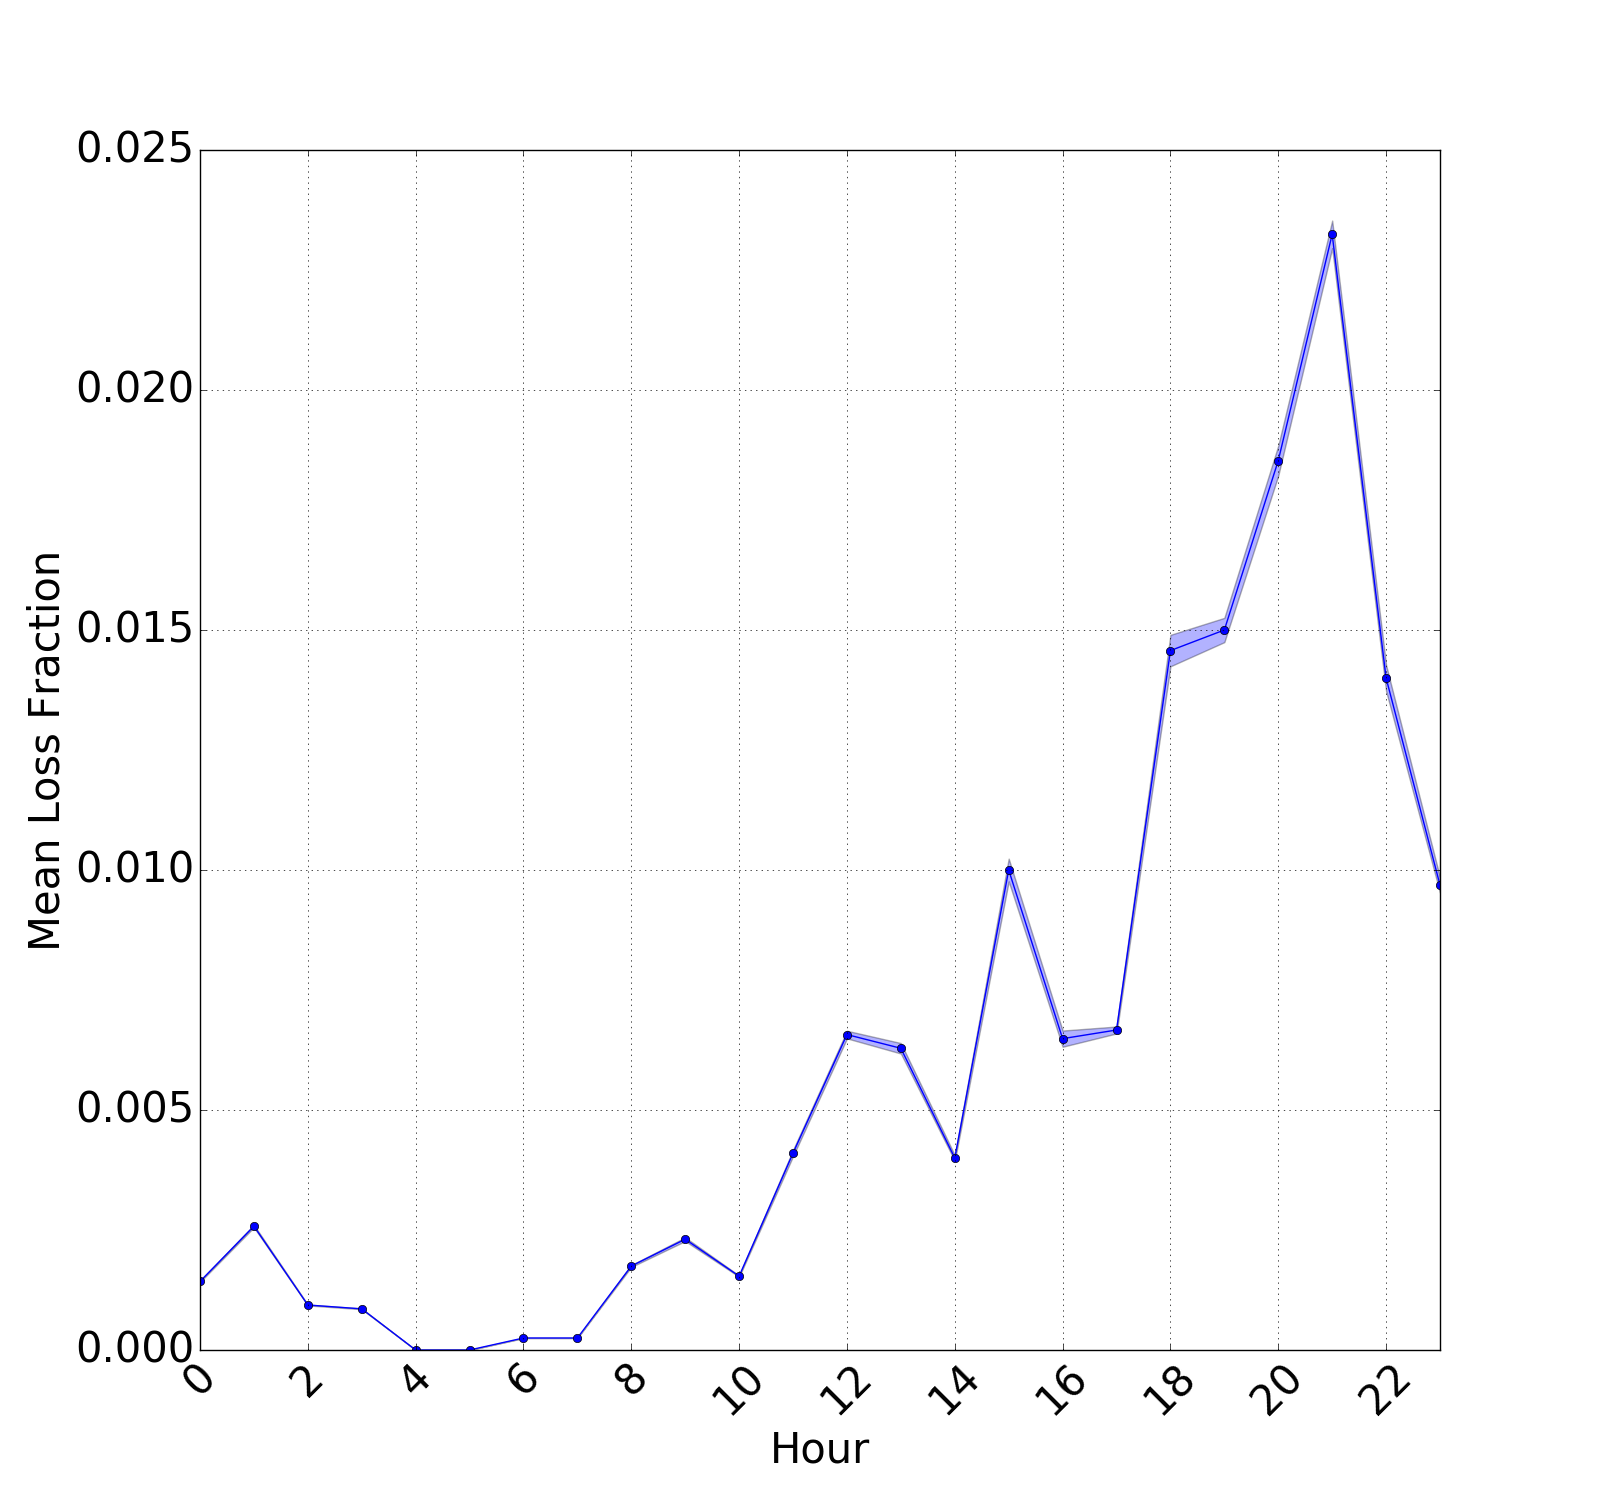
\includegraphics[width=1.0\textwidth]{./figures/dataset/ts/mean_per_hour_in_a_day_NHODTCSRV04_64:66:B3:50:06:90.png}
            \caption{Mean and variance per hour}
        \end{subfigure}%~
        \begin{subfigure}[b]{0.55\textwidth}
            \centering
            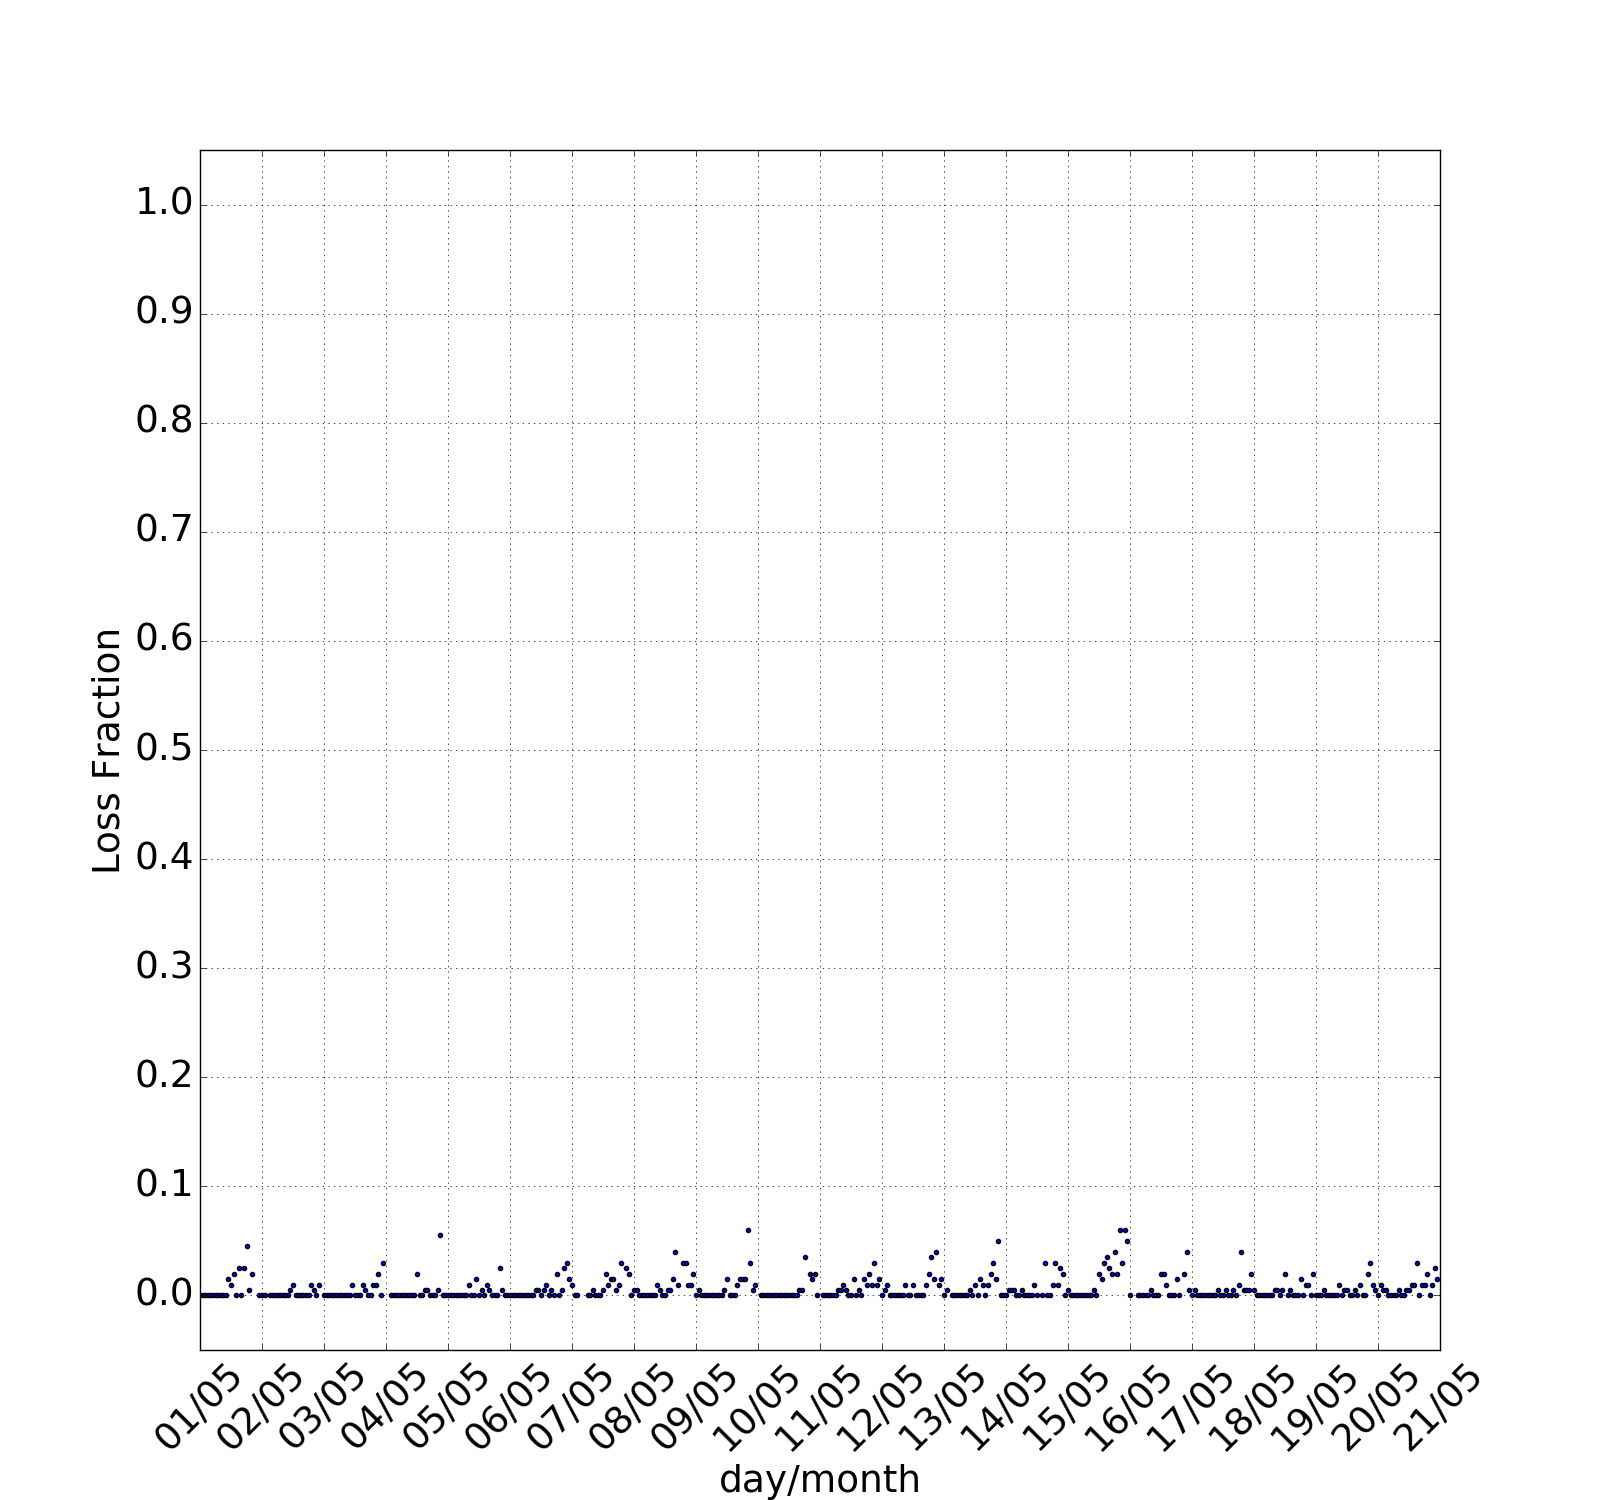
\includegraphics[width=1.0\textwidth]{./figures/dataset/ts/ts_NHODTCSRV04_64:66:B3:50:06:90.png}
            \caption{Time series}
        \end{subfigure}
    }
    \caption{Client 4}
    \label{fig:mean_day_hour_ts}
\end{figure}

With a visual analysis, as in the previous plots, it is possible to observe different time series and change points patterns.

\section{Change Points Dataset}

\subsection{Methodology}

There are several approaches to construct a change points dataset. Some works create simulated time series, in which distinct segments are sampled by the same generative model with different parameters \cite{change_point_detection_in_time_series_data_by_relative_density_ratio_estimation}. In general, this type of data is more easily handled by change point detection algorithms, since some methods assume the same models used in the dataset building process. Also, real data can have complex characteristics that are difficult to be reproduced by generative models. Another strategy is to join segments from different real time series \cite{inertial_hidden_markov_models_modeling_change_in_multivariate_time_series}. However, this can introduce unreal change points scenarios.

When the latent information of the time series are available, and if there is a complete knowledge of what configurations changes in the latent state impact data, it is possible to check the change points only analyzing this underlying information. As an example, consider a time series that represents the cardiac frequency of a soccer player during a match. Also, consider that in this controlled environment, the only causes of changes in the cardiac frequency are the variations of physical activities, such as start or stop running. Therefore, it is possible to use the times in which a player changed his movement behavior as the change points, whithout even analyzing the time series. However, in the application domain of the present work, this approach would be impractical. First, this would need the expertise of how the configurations of network topology, routers congestion, physical equipment problems, among other features, affect the loss fraction. Second, this kind of information is absent in the dataset, and would be too complex to collect it.

The approach followed in this work was to use visual classifications, as it was done in \cite{learning_sparse_penalties_for_change_point_detection_using_max_margin_interval_regression}. An application domain expert was exposed to a set of time series, and visually indicated his opinion about the change points locations. It is known that visual inspection methods can bring erroneous conclusions \cite{leveraging_cloud_data_to_mitigate_user_experience_from_breaking_bad}, and also amplify subjectivity, however, it was the best alternative considering the data availability and the objective of working with real data.

Through a web system the user freely marked the change points with a mouse. The fact that data is not regularly sampled in time could bring an unwanted visual change perception. Therefore, the X axis of the displayed time series represented only the temporal order of the measures.

A single specialist classified all time series. This person has experience with network measurements and statistical modeling, however, without background in change point detection. The user could take any time to make a classification, and it was able to access the system in different days. Additionally, it was provided a set of tips to the specialist:

\begin{itemize}
    \item In the case of packet loss fraction, mean changes between 0 and 0.1 are more sensible to the end users.
    \item The time axis only represents the temporal order of the measurements. However, in general, consecutive points in time axis are separated by 30 minutes.
    \item Outlier is not a statistical change. An outlier is an observation that lies outside the overall pattern of a distribution.
\end{itemize}

To provide a clear visualization, the change points dataset was composed by time series with 10 days of data. Therefore, each time series of the previous dataset was split in two, one from 01/may/2016 to 10/may/2016, and other from 11/may/2016 to 20/may/2016. Also, it was selected only the ones that have at least 85\% of the maximum possible number of points during the specified period, considering that data is sampled at most two times in a hour. Change points can be interpreted as rare events in this dataset, and most data streams have almost all measures with zero losses. Therefore, to increase the dataset entropy, it was only selected time series that have at least one window of length 48 with more than 5 measures with loss fraction larger than 0.01. These filters resulted in 522 time series.

Figure~\ref{fig:survey_system} presents a system snapshot. The vertical red line means that the user marked a change point in that position.

\begin{figure}[H]
    \centering
    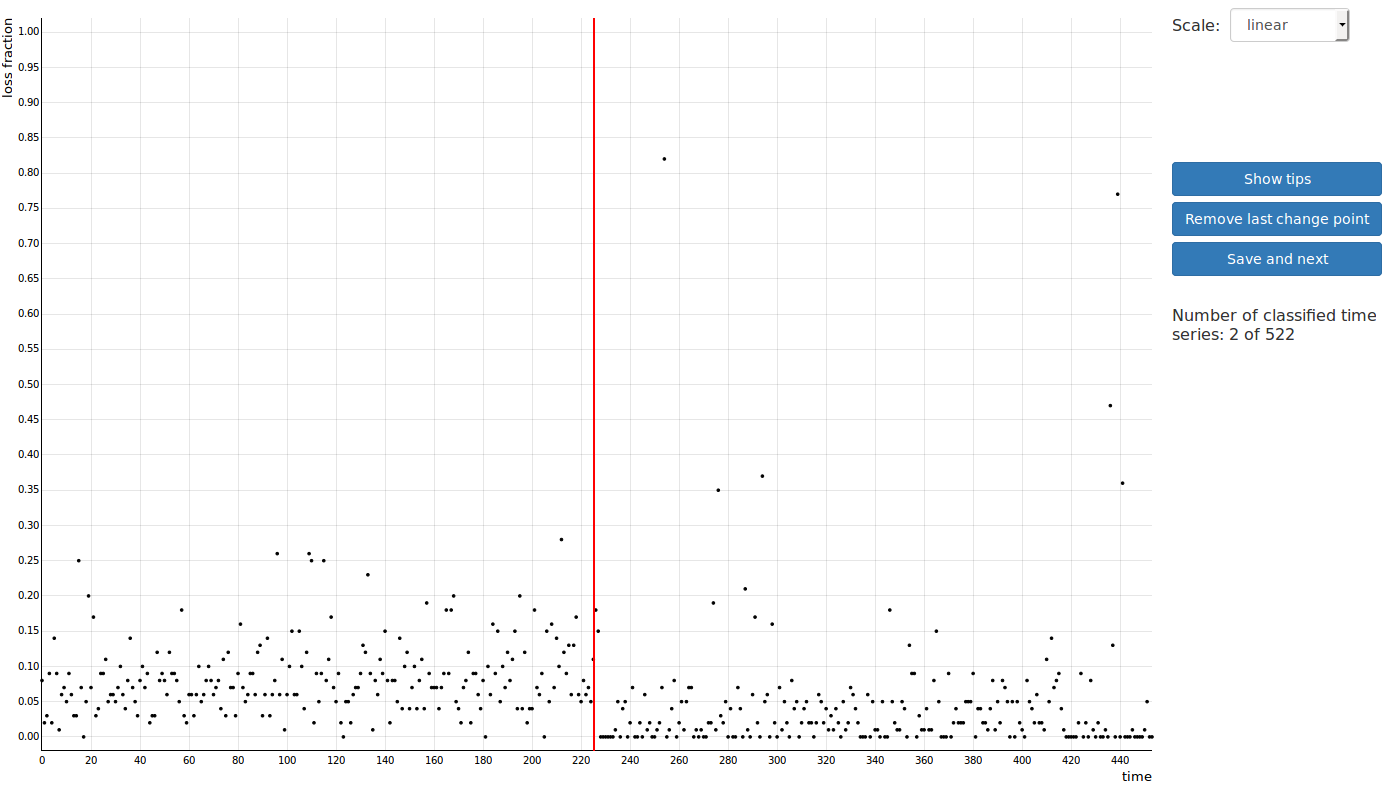
\includegraphics[width=\linewidth]{./figures/dataset/cp/survey_system.png}
    \caption{Survey system snapshot}
    \label{fig:survey_system}
\end{figure}%

\subsection{Descriptive Analysis}

The resulted dataset consists of 522 time series, 241470 measures, and 866 change points. The change point detection problem can be interpreted as a binary classification task, in which points are labeled as change points or not change points. These two classes are highly unbalanced in this dataset, since only 0.4\% of the points are change points. 

Next, in Figure~\ref{fig:cps_per_ts}, is presented the number of change points per time series distribution.

\begin{figure}[H]
    \centering
    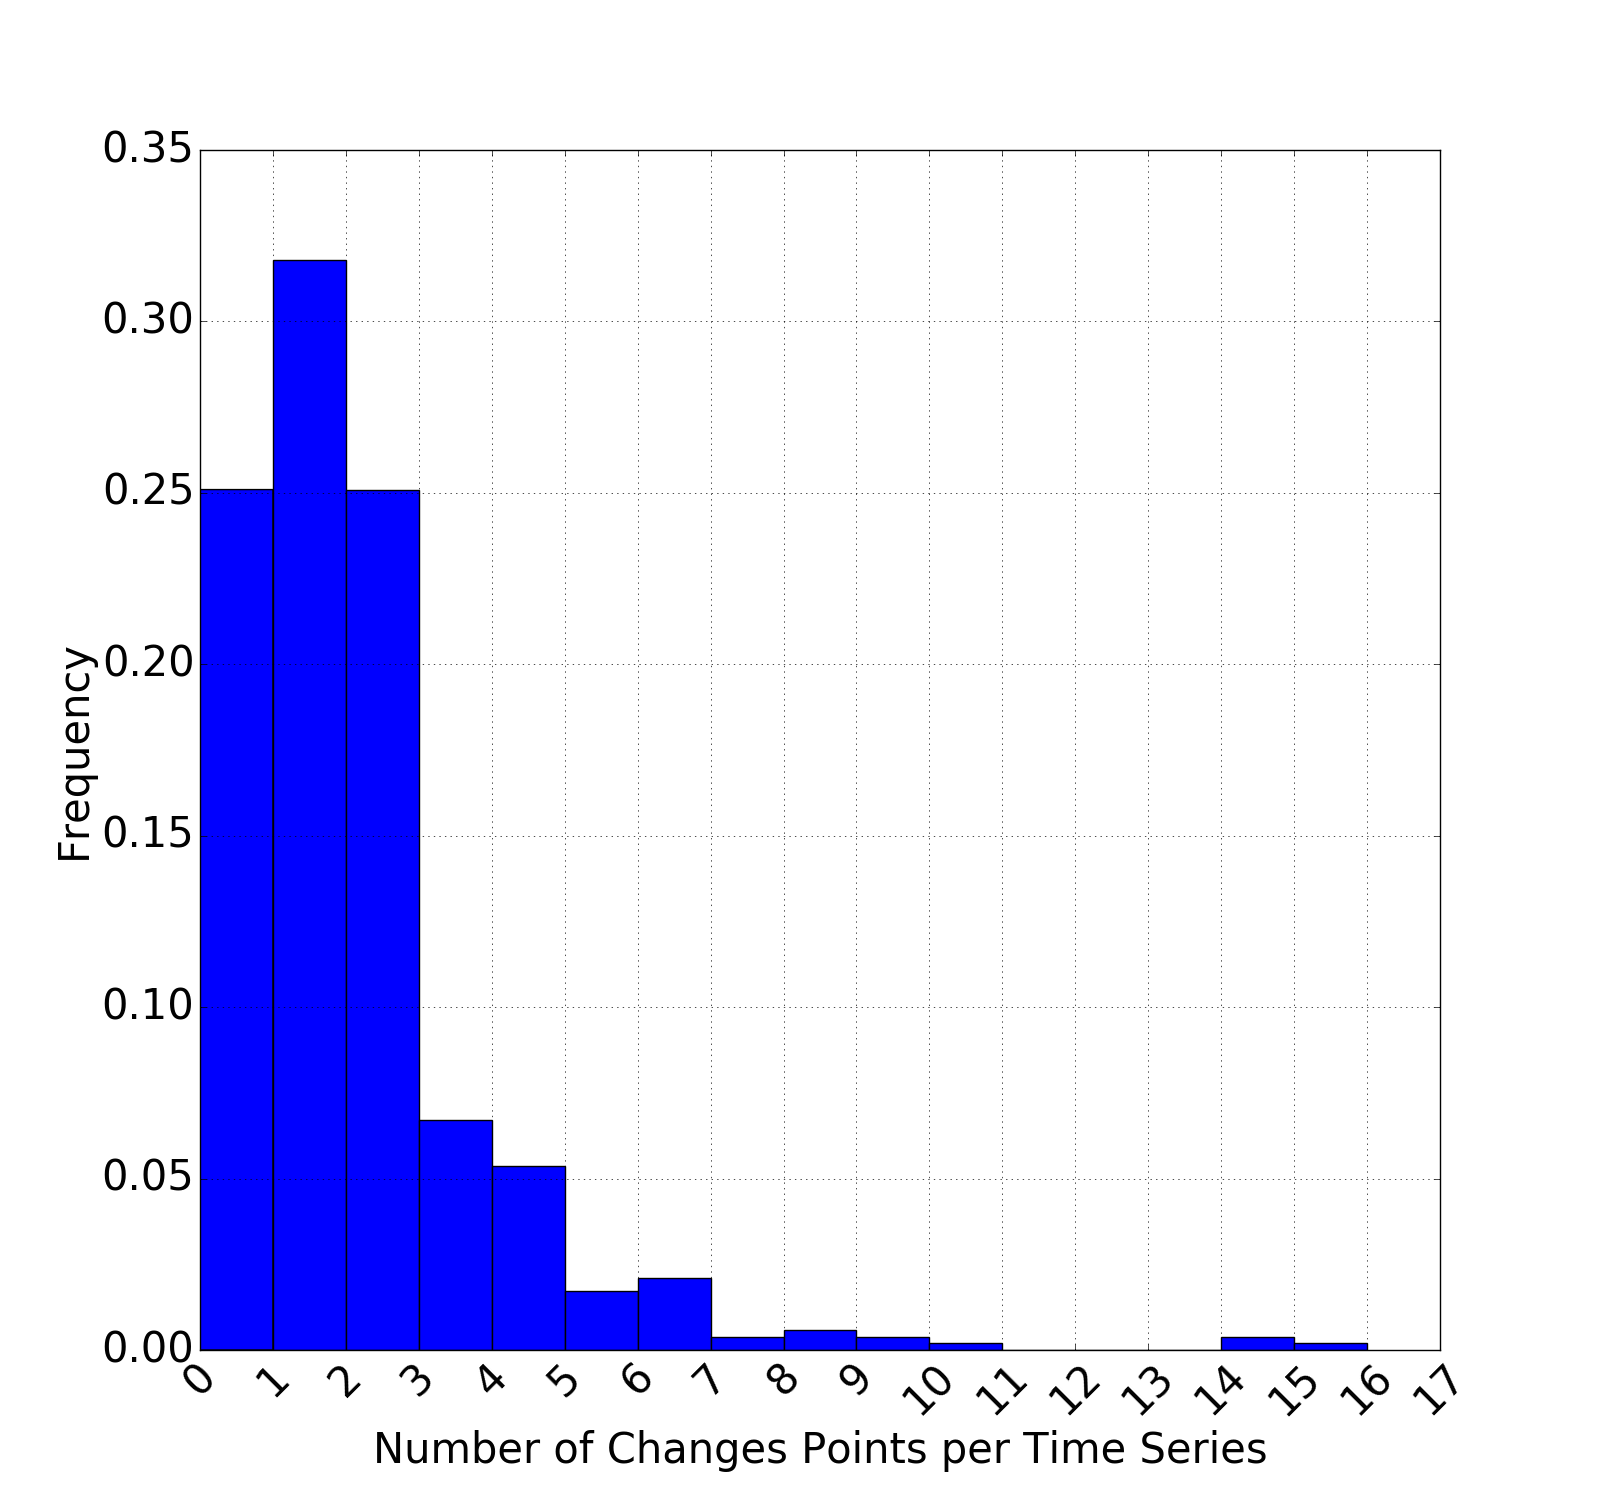
\includegraphics[width=0.6\linewidth]{./figures/dataset/cp/cps_per_ts.png}
    \caption{Number of change points per time series distribution}
    \label{fig:cps_per_ts}
\end{figure}%

Figure~\ref{fig:segs_length} presents the segment length distribution, conditioning on data streams that have at least one change point. Since the time series have points past the first segment, and also in the future of the last, this analysis dismissed the first and last windows. This avoids incorrect conclusions about how much time a client stands with the same pattern.

\begin{figure}[H]
    \centering
    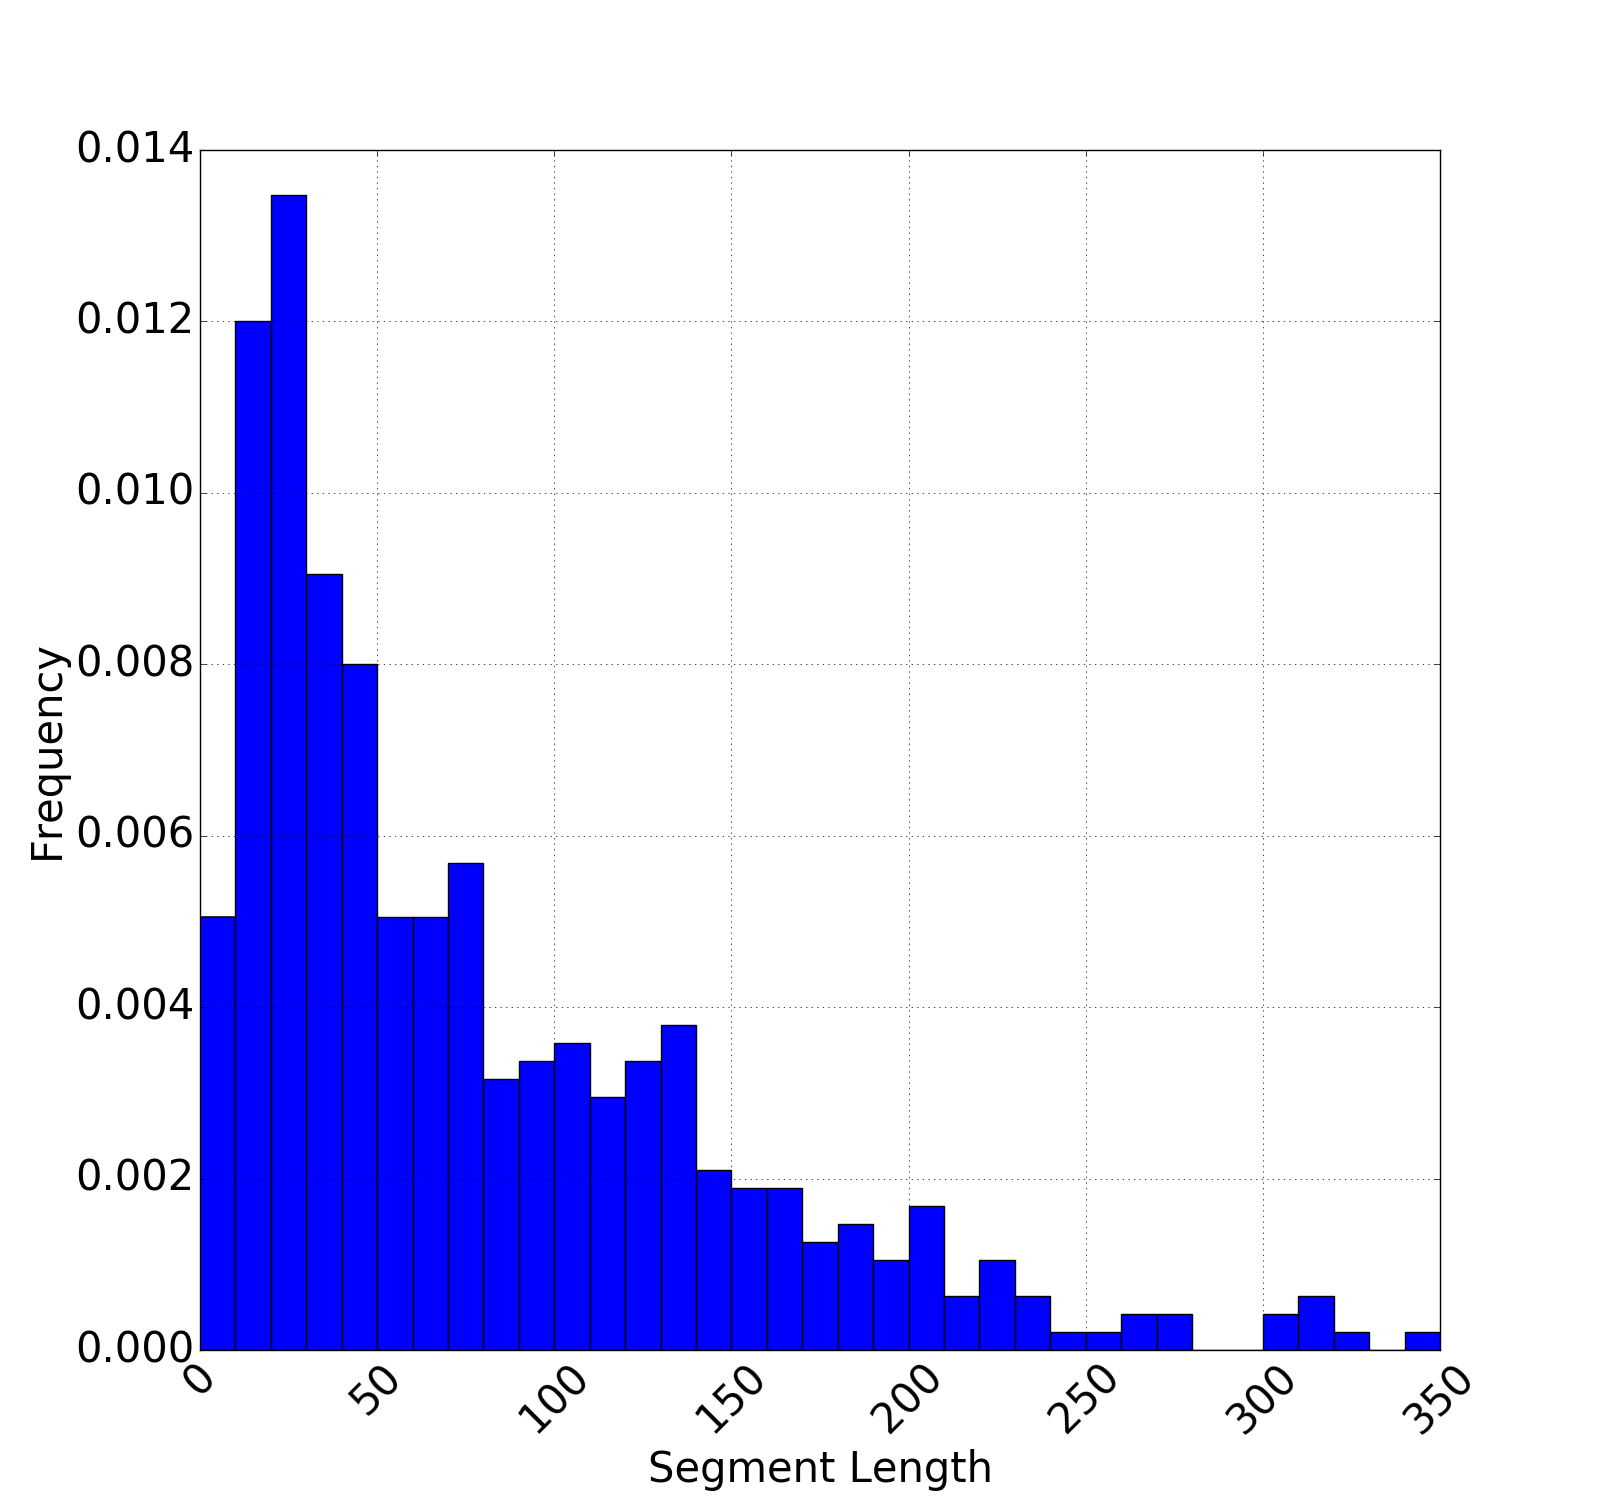
\includegraphics[width=0.6\linewidth]{./figures/dataset/cp/middle_segment_length.png}
    \caption{Segment length distribution. Bins of size 10.}
    \label{fig:segs_length}
\end{figure}%

In Figure~\ref{fig:consecutive_segs_comparison} is made a comparison between consecutive segments, presenting the absolute mean difference and the discrete Hellinger distance distributions.

\begin{figure}[H]
    \makebox[\linewidth][c]{%
        \centering
        \begin{subfigure}[b]{0.55\textwidth}
            \centering
            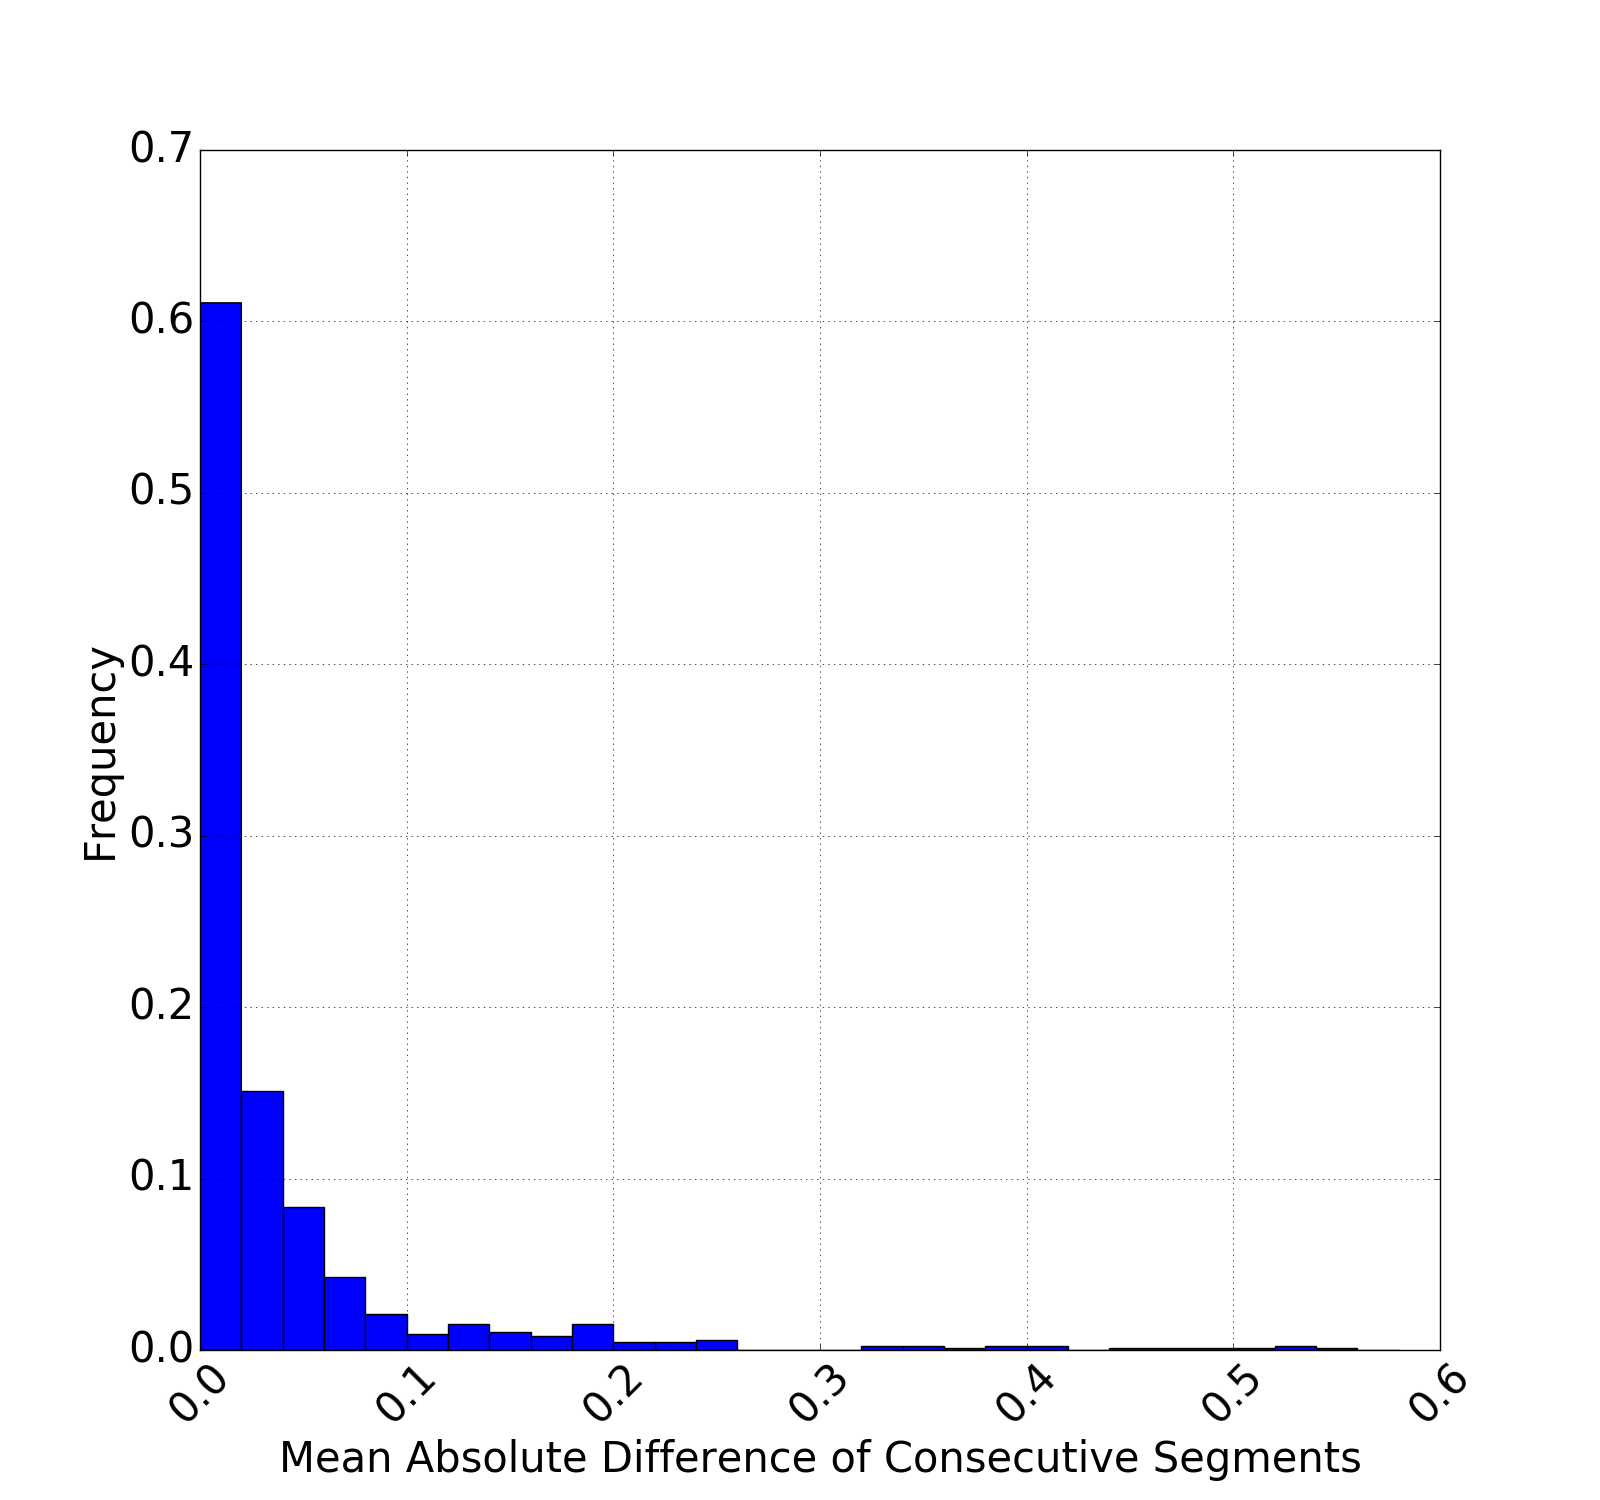
\includegraphics[width=1.0\textwidth]{./figures/dataset/cp/mean_abs_diff_consecutive_segs.png}
            \caption{Absolute mean difference}
        \end{subfigure}%~
        \begin{subfigure}[b]{0.55\textwidth}
            \centering
            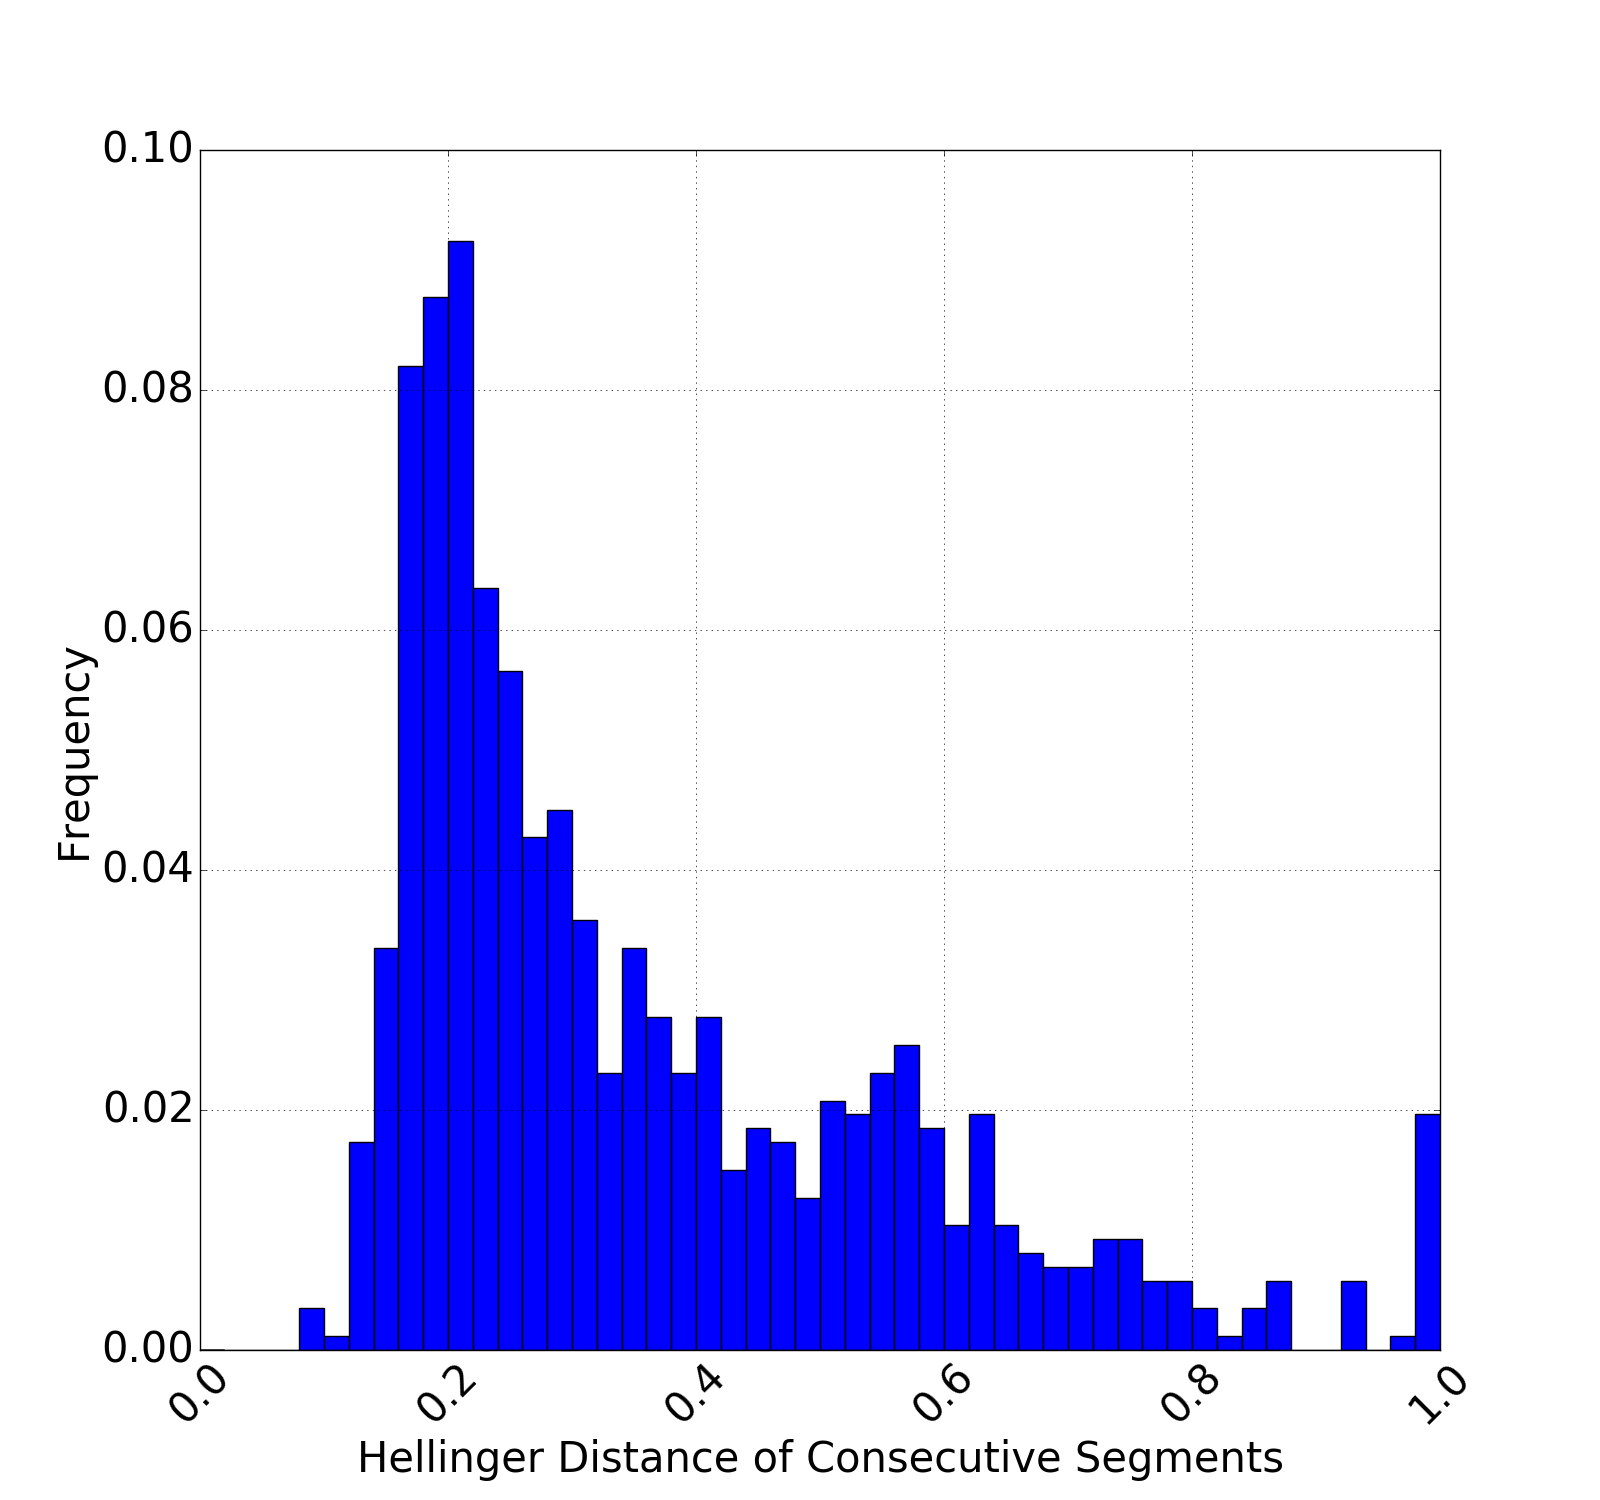
\includegraphics[width=1.0\textwidth]{./figures/dataset/cp/hellinger_consecutive_segs.png}
            \caption{Hellinger distance}
        \end{subfigure}
    }
    \caption{Consecutive segments comparison. Bins of size 0.02.}
    \label{fig:consecutive_segs_comparison}
\end{figure}
